\documentclass{article}

  % packages
    % basic stuff for rendering math
    \usepackage[letterpaper, top=1in, bottom=1in, left=1in, right=1in]{geometry}
    \usepackage[utf8]{inputenc}
    \usepackage[english]{babel}
    \usepackage{amsmath} 
    \usepackage{amssymb}
    \usepackage{bookmark}

    % extra math symbols and utilities
    \usepackage{mathtools}        % for extra stuff like \coloneqq
    \usepackage{mathrsfs}         % for extra stuff like \mathsrc{}
    \usepackage{centernot}        % for the centernot arrow 
    \usepackage{bm}               % for better boldsymbol/mathbf 
    \usepackage{enumitem}         % better control over enumerate, itemize
    \usepackage{hyperref}         % for hypertext linking
    \usepackage{xr-hyper}
    \usepackage{fancyvrb}          % for better verbatim environments
    \usepackage{newverbs}         % for texttt{}
    \usepackage{xcolor}           % for colored text 
    \usepackage{listings}         % to include code
    \usepackage{lstautogobble}    % helper package for code
    \usepackage{parcolumns}       % for side by side columns for two column code
    \usepackage{algorithm}
    \usepackage{algpseudocode}
    \usepackage{bbm}
    \algblock{Class}{EndClass}

    % page layout
    \usepackage{fancyhdr}         % for headers and footers 
    \usepackage{uniquecounter}
    \usepackage{lastpage}         % to include last page number in footer 
    \usepackage{parskip}          % for no indentation and space between paragraphs   
    \usepackage[T1]{fontenc}      % to include \textbackslash
    \usepackage{footnote}
    \usepackage{etoolbox}

    % for custom environments
    \usepackage{tcolorbox}        % for better colored boxes in custom environments
    \tcbuselibrary{breakable}     % to allow tcolorboxes to break across pages

    % figures
    \usepackage{pgfplots}
    \pgfplotsset{compat=1.18}
    \usepackage{float}            % for [H] figure placement
    \usepackage{tikz}
    \usepackage{tikz-cd}
    \usepackage{circuitikz}
    \usetikzlibrary{arrows, arrows.meta}
    \usetikzlibrary{positioning}
    \usetikzlibrary{calc}
    \usepackage{graphicx}
    \usepackage{caption} 
    \usepackage{subcaption}
    \captionsetup{font=small} 

    % for tabular stuff 
    \usepackage{dcolumn}

    \usepackage[nottoc]{tocbibind}
    \pdfsuppresswarningpagegroup=1
    \hfuzz=5.002pt                % ignore overfull hbox badness warnings below this limit

  % New and replaced operators
    \DeclareMathOperator{\Tr}{Tr}
    \DeclareMathOperator{\Sym}{Sym}
    \DeclareMathOperator{\Span}{span}
    \DeclareMathOperator{\elbo}{ELBO}
    \DeclareMathOperator{\std}{std}
    \DeclareMathOperator{\Cov}{Cov}
    \DeclareMathOperator{\Var}{Var}
    \DeclareMathOperator{\Corr}{Corr}
    \DeclareMathOperator{\pos}{pos}
    \DeclareMathOperator*{\argmin}{\arg\!\min}
    \DeclareMathOperator*{\argmax}{\arg\!\max}
    \newcommand{\qed}{\hfill$\blacksquare$}     % I like QED squares to be black

  % Custom Environments
    \newtcolorbox[auto counter, number within=section]{question}[1][]
    {
      colframe = orange!25,
      colback  = orange!10,
      coltitle = orange!20!black,  
      breakable, 
      title = \textbf{Question \thetcbcounter ~(#1)}
    }

    \newtcolorbox[auto counter, number within=section]{exercise}[1][]
    {
      colframe = teal!25,
      colback  = teal!10,
      coltitle = teal!20!black,  
      breakable, 
      title = \textbf{Exercise \thetcbcounter ~(#1)}
    }
    \newtcolorbox[auto counter, number within=section]{solution}[1][]
    {
      colframe = violet!25,
      colback  = violet!10,
      coltitle = violet!20!black,  
      breakable, 
      title = \textbf{Solution \thetcbcounter}
    }
    \newtcolorbox[auto counter, number within=section]{lemma}[1][]
    {
      colframe = red!25,
      colback  = red!10,
      coltitle = red!20!black,  
      breakable, 
      title = \textbf{Lemma \thetcbcounter ~(#1)}
    }
    \newtcolorbox[auto counter, number within=section]{theorem}[1][]
    {
      colframe = red!25,
      colback  = red!10,
      coltitle = red!20!black,  
      breakable, 
      title = \textbf{Theorem \thetcbcounter ~(#1)}
    } 
    \newtcolorbox[auto counter, number within=section]{corollary}[1][]
    {
      colframe = red!25,
      colback  = red!10,
      coltitle = red!20!black,  
      breakable, 
      title = \textbf{Corollary \thetcbcounter ~(#1)}
    } 
    \newtcolorbox[auto counter, number within=section]{proof}[1][]
    {
      colframe = orange!25,
      colback  = orange!10,
      coltitle = orange!20!black,  
      breakable, 
      title = \textbf{Proof. }
    } 
    \newtcolorbox[auto counter, number within=section]{definition}[1][]
    {
      colframe = yellow!25,
      colback  = yellow!10,
      coltitle = yellow!20!black,  
      breakable, 
      title = \textbf{Definition \thetcbcounter ~(#1)}
    } 
    \newtcolorbox[auto counter, number within=section]{example}[1][]
    {
      colframe = blue!25,
      colback  = blue!10,
      coltitle = blue!20!black,  
      breakable, 
      title = \textbf{Example \thetcbcounter ~(#1)}
    } 
    \newtcolorbox[auto counter, number within=section]{code}[1][]
    {
      colframe = green!25,
      colback  = green!10,
      coltitle = green!20!black,  
      breakable, 
      title = \textbf{Code \thetcbcounter ~(#1)}
    } 
    \newtcolorbox[auto counter, number within=section]{algo}[1][]
    {
      colframe = green!25,
      colback  = green!10,
      coltitle = green!20!black,  
      breakable, 
      title = \textbf{Algorithm \thetcbcounter ~(#1)}
    } 
    \definecolor{cverbbg}{gray}{0.93}
    \newenvironment{cverbatim}
      {\SaveVerbatim{cverb}}
      {\endSaveVerbatim
        \flushleft\fboxrule=0pt\fboxsep=.5em
        \colorbox{cverbbg}{%
          \makebox[\dimexpr\linewidth-2\fboxsep][l]{\BUseVerbatim{cverb}}%
        }
        \endflushleft
    }

    \definecolor{dkgreen}{rgb}{0,0.6,0}
    \definecolor{gray}{rgb}{0.5,0.5,0.5}
    \definecolor{mauve}{rgb}{0.58,0,0.82}
    \definecolor{lightgray}{gray}{0.93}
    \renewcommand{\algorithmiccomment}[1]{\hfill$\triangleright$\textcolor{blue}{#1}}

    % default options for listings (for code)
    \lstset{
      autogobble,
      frame=ltbr,
      language=Python,                           % the language of the code
      aboveskip=3mm,
      belowskip=3mm,
      showstringspaces=false,
      columns=fullflexible,
      keepspaces=true,
      basicstyle={\small\ttfamily},
      numbers=left,
      firstnumber=1,                        % start line number at 1
      numberstyle=\tiny\color{gray},
      keywordstyle=\color{blue},
      commentstyle=\color{dkgreen},
      stringstyle=\color{mauve},
      backgroundcolor=\color{lightgray}, 
      breaklines=true,                      % break lines
      breakatwhitespace=true,
      tabsize=3, 
      xleftmargin=2em, 
      framexleftmargin=1.5em, 
      stepnumber=1
    }

  % Page style
    \pagestyle{fancy}
    \fancyhead[L]{CNN}
    \fancyhead[C]{Muchang Bahng}
    \fancyhead[R]{Spring 2023} 
    \fancyfoot[C]{\thepage / \pageref{LastPage}}
    \renewcommand{\footrulewidth}{0.4pt}          % the footer line should be 0.4pt wide
    \renewcommand{\thispagestyle}[1]{}  % needed to include headers in title page
%    \renewcommand{\thefootnote}{\arabic{footnote}}

  % external documents 
    \externaldocument[algo-]{../../Computer_Science/DSA/paper}[../../Computer_Science/DSA/paper.pdf]

\begin{document}

\tikzset{every picture/.style={line width=0.75pt}} 

\title{Convolutional Neural Networks}
\author{Muchang Bahng}
\date{Spring 2023}

\maketitle
\tableofcontents
\pagebreak 


This covers computability theory, complexity theory, and automata theory. 
Alphabet. Boolean logic

 
\section{Convolution} 

  Convolutional networks work with images, so let's introduce a nice way to represent them as vectors. 

  \begin{definition}[Image]
    An image is a vector in some tensor product space. More specifically, avoiding the technicality that each pixel element is bounded and discrete, 

    \begin{enumerate}
      \item A \textbf{grayscale image} of resolution of $H \times W$ is a vector in $\mathbb{R}^{H} \otimes \mathbb{R}^{W}$. 
      \item An \textbf{image} with $C$ channels of the same resolution is an element of $\mathbb{R}^{C} \otimes \mathbb{R}^H \otimes \mathbb{R}^W$. 
      \item A \textbf{video} with $C$ channels and of the same resolution is an element of $\mathbb{R}^T \otimes \mathbb{R}^C \otimes \mathbb{R}^H \otimes \mathbb{R}^W$, where $T$ is the time dimension which is usually represented in some discrete frames.
    \end{enumerate} 
    Usually, we denote the height/width as the \textbf{spatial dimension}, the colors and the \textbf{channel dimension}, and time as the \textbf{temporal dimension}.\footnote{Everything we talked about so far applies to images when treated as vectors. In fact, so far we have been interpreting images of size $(C, H, W)$ through the isomorphism $\phi: \mathbb{R}^{C} \otimes \mathbb{R}^H \otimes \mathbb{R}^W \rightarrow \mathbb{R}^{C \times H \times W}$ that essentially ``unravels" the image. }
  \end{definition}

  Note that the terminology above is general convention, and tensors of arbitrary shape may exist that encode---say time over two dimensions. So far, we have seen the power of multilayer perceptrons and their predictive ability on moderately sized vectors. In fact, if we process the MNIST with a simple MLP of 2 layers and 512 nodes each, we can easily get $95\%$ accuracy within 10 epochs. However, these MNIST pictures are extremely low resolution, at $1 \times 28 \times 28$, and for even moderately sized images we can that there is a huge blowup of parameters needed. \footnote{For example, an RGB image that is $3 \times 1024 \times 1024$ would have ~3m parameters, and then defining a dense linear map to even 1000 dimensions would take 3 billion parameters. Given that 32-bit floating point is $4$ bytes, this already takes up 12GB of memory just to load the network.} Clearly, this is not efficient, and so the only way to move on is to create a sparser representation of the network. Therefore, can we create a sparser representation of a linear map that does sacrifice too much expressibility for memory? With convolutional kernels\footnote{Note that this is completely different than the kernels mentioned in supervised learning, with support vector machines and RKHS.}, the answer is yes. In 1994, Yann LeCunn and Yoshua Bengio in Bell Labs published \cite{cnn} which introduced the \textit{convolutional neural network}. 

  The only layer know is a fully-connected layer. Now we will learn about our second type of layer. 

  \begin{definition}[1D Convolutional Layer]
    A \textbf{1D convolutional operator/layer} of 
    \begin{enumerate}
      \item input channels $C_{\mathrm{in}}$ 
      \item output channels $C_{\mathrm{out}}$ 
      \item kernel size $K$ 
      \item stride $S$
    \end{enumerate}
    is an operator $\phi: \mathbb{R}^{C_{\mathrm{in}}} \times \mathbb{R}^L \rightarrow \mathbb{R}^{C_{\mathrm{out}}} \times \mathbb{R}^{L_{\mathrm{out}}}$, where $C$ is the channel dimension and $L$ is the spatial dimension. We can view 
    \begin{equation}
      \phi(x)_{c, i} = \sum_{} 
    \end{equation}
  \end{definition}

  \begin{definition}[2D Convolutional Layer]
    A \textbf{convolutional operator/layer} of 
    \begin{enumerate}
      \item size 
    \end{enumerate}
  \end{definition}

  \begin{definition}[3D Convolutional Layer]
    A \textbf{convolutional operator/layer} of 
    \begin{enumerate}
      \item size 
    \end{enumerate}
  \end{definition}

  \begin{figure}[H]
    \centering 
    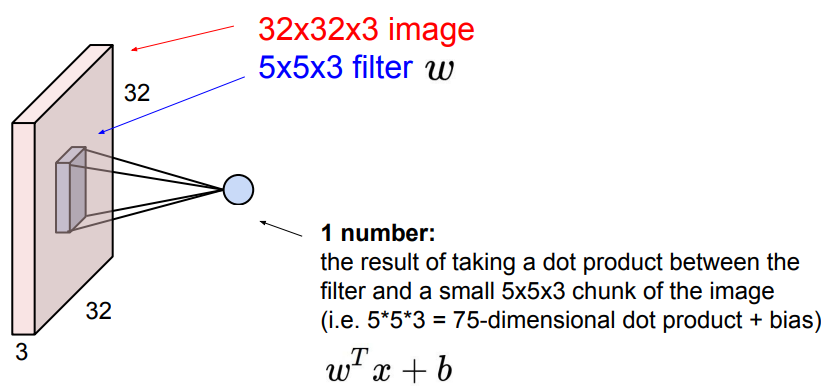
\includegraphics[scale=0.35]{img/kernel1.png}
    \caption{} 
    \label{fig:kernel1}
  \end{figure}

  \begin{figure}[H]
    \centering 
    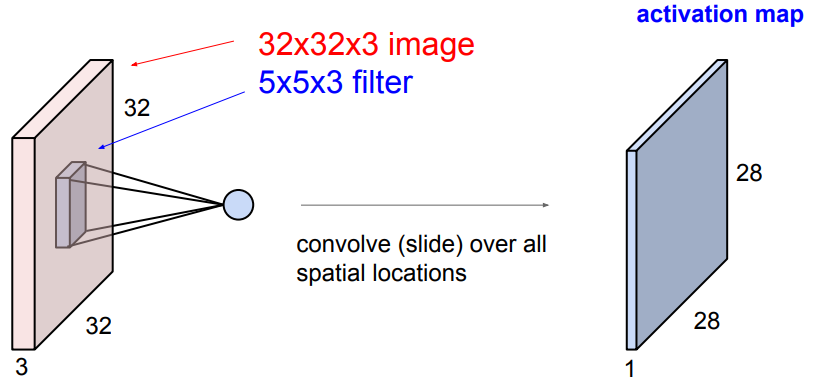
\includegraphics[scale=0.35]{img/kernel2.png}
    \caption{} 
    \label{fig:kernel2}
  \end{figure}

  \begin{figure}[H]
    \centering 
    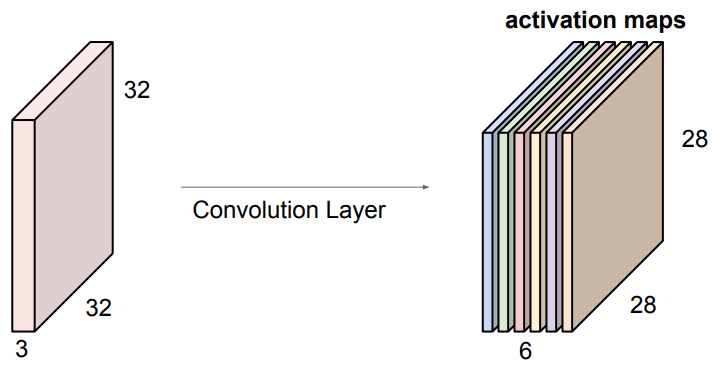
\includegraphics[scale=0.35]{img/kernel3.png}
    \caption{} 
    \label{fig:kernel3}
  \end{figure}

  \begin{definition}[Convolutional Kernel]
    A \textbf{convolution operator} on a vector space $V$ representing an image space is simply a special type of linear map that is parameterized by a much smaller set of numbers, stored within a \textbf{kernel} or \textbf{filter}. In all honesty, it is much easier to go through examples to see how they work, so in this definition I will focus more on describing the hyperparameters. Given an image of shape $(C, H, W)$, the convolution is essentially a sliding window that computes a dot product between the kernel and the window that the kernel covers over the image. 
    \begin{enumerate}
      \item The sliding window size is $(W_{ker}, H_{ker})$, which is conventionally square but does not need to be. 

      \item This sliding window must compute over all channels, so in fact it is of shape $(C_{in}, W_{ker}, H_{ker})$. This would generate one output channel image. 

      \item Multiple kernels can be used concurrently to generate different channel images. Therefore, if we want to have a collection of $C_{\text{out}}$ outputs that are extracted from each kernel, our total kernel would be a collection of $C_{out}$ kernels of shape $(C_{in}, W_{ker}, H_{ker}, C_{out})$. Therefore, the total equation is 
      \begin{equation}
        (X \ast K)_{f, i, j} \coloneqq \sum_c \sum_{p, q} X_{c, i + p, j + q} \cdot K_{c, p, q, f} + b_{f, i, j}
      \end{equation}

      where $c$ is the channel index, $p, q$ are the location indices, $f$ is the output channel index, and $b$ is some bias term. 

      \item The stride parameter $s$ can also be set to determine the stride of the kernel $\mathcal{K}$. 

      \item Another thing to note is that the output image of a kernel would be slightly smaller than the input image, since the kernel cannot go over the edge. However, there are padding schemes to preserve the original dimensions. 
    \end{enumerate}
    From the equation above, we can see that a convolutional layer, assuming that it has full padding, is a linear map  
    \begin{equation}
      \mathcal{K} : \mathbb{R}^{C_{in}} \otimes \mathbb{R}^H \otimes \mathbb{R}^W \rightarrow \mathbb{R}^{C_{out}} \otimes \mathbb{R}^H \otimes \mathbb{R}^W
      \label{eq:conv_mapping}
    \end{equation}
    The vector space of linear maps mapping between these two spaces has $C_{in} H^2 W^2 C_{out}$ dimensions, which is extremely large, but parameterizing $\mathcal{K}$ with this matrix reduces the set of relevant convolutional maps to a subspace that is $(1 + C_{in} H_{ker} W_{ker}) C_{out}$ dimensional (with the $+1$ due to a bias term, making this an affine map). This is essentially what a convolution is: sparse matrix multiplication, and there is nothing else that makes it different from a classical feedforward neural network. It's just computationally efficient matrix multiplication for high-dimensional vectors. 
  \end{definition}

  In addition to computational efficiency and weight sharing, convolutional operators capitalize on the principle of \textbf{locality}, i.e. that pixels are directly related to adjacent pixels. For example, a pixel representing a portion of a dog's ear would not be related to the background, but the color and positioning should be related to the dog's face, which may be within a certain neighborhood around. This has been shown to be similar to the human visual system and is thus well motivated. 

  Though this next topic has more to do with classical image processing than computer vision, there are a surprising number of features that these convolutional filters can extract from an image. By treating them as a discretized form of a partial derivative (as the vertical and horizontal edge detection) or as the Hessian operator (sharpening), we can extract many features from them.  

  \begin{example}[Blurs, Edge Detection]
    Given the original image below, we show various convolutional filters applied on the image. Note that the kernel matrix may have the property that all of its entries sum to $1$, meaning that on average, the expected value of the brightness of each pixel will be $0$, and the values will be left unchanged on average. However, this is not a requirement.  
    \begin{align*}
      \mathrm{Original} = \begin{bmatrix} 1 & 0 & 0 & 0 & 0 \\ 0 & 1 & 0 & 0 & 0 \\ 0 & 0 & 1 & 0 & 0 \\ 0 & 0 & 0 & 1 & 0 \\ 0 & 0 & 0 & 0 & 1 \end{bmatrix} & 
      \mathrm{Mean} = \frac{1}{25} \begin{bmatrix} 1 & 1 & 1 & 1 & 1 \\ 1 & 1 & 1 & 1 & 1 \\ 1 & 1 & 1 & 1 & 1 \\ 1 & 1 & 1 & 1 & 1 \\ 1 & 1 & 1 & 1 & 1 \end{bmatrix} & 
      \mathrm{Gaussian} = \frac{1}{273} \begin{bmatrix} 1 & 4 & 7 & 4 & 1 \\ 4 & 16 & 26 & 16 & 4 \\ 7 & 26 & 41 & 26 & 7 \\ 4 & 16 & 26 & 16 & 4 \\ 1 & 4 & 7 & 4 & 1 \end{bmatrix} \\   
      \mathrm{Sharpen} = \begin{bmatrix} 0 & -1 & 0 \\ -1 & 5 & -1 \\ 0 & -1 & 0 \end{bmatrix} & 
      \mathrm{Horizontal} = \begin{bmatrix} -1 & 0 & 1 \\ -2 & 0 & 2 \\ -1 & 0 & 1 \end{bmatrix} & 
      \mathrm{Vertical} = \begin{bmatrix} -1 & -2 & -1 \\ 0 & 0 & 0 \\ 1 & 2 & 1 \end{bmatrix} 
    \end{align*}

    These filters visually output the following images. Note that these filters are each acting on the image by acting individually on each channel and then combining the 3 outputs to create the new RGB image. 
    \begin{figure}[H]
      \centering
      \begin{subfigure}[b]{0.32\textwidth}
      \centering
          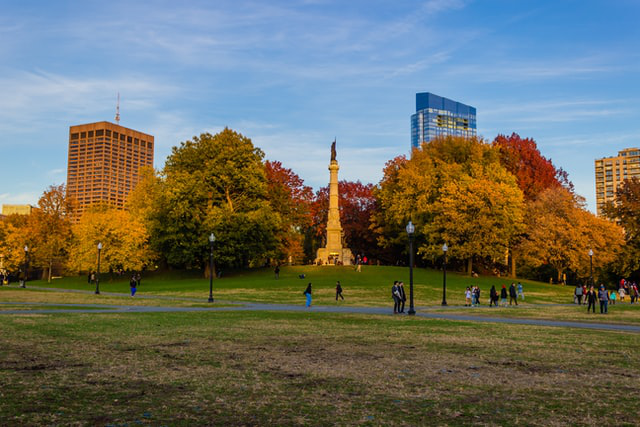
\includegraphics[width=\textwidth]{img/Park_Full.png}
          \caption{Original image. }
          \label{fig:original_image}
      \end{subfigure}
      \begin{subfigure}[b]{0.32\textwidth}
      \centering
          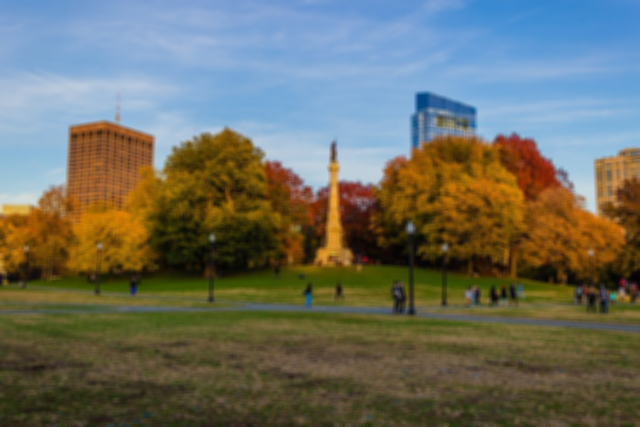
\includegraphics[width=\textwidth]{img/Mean_Blur.png}
          \caption{$5 \times 5$ mean blur applied. }
          \label{fig:mean_blur_image}
      \end{subfigure}
      \begin{subfigure}[b]{0.32\textwidth}
      \centering
          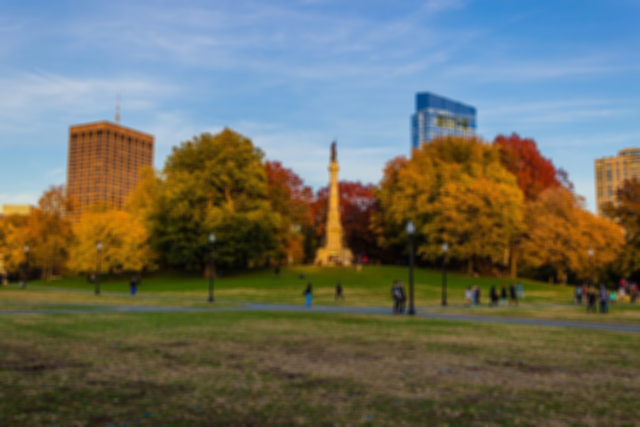
\includegraphics[width=\textwidth]{img/Gaussian_Blur.png}
          \caption{$5 \times 5$ Gaussian blur applied. }
          \label{fig:normal_blur_image}
      \end{subfigure}
      
      \begin{subfigure}[b]{0.32\textwidth}
      \centering
          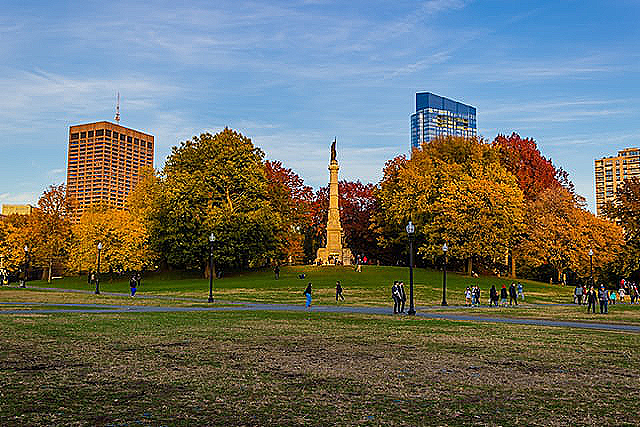
\includegraphics[width=\textwidth]{img/Sharpen.png}
          \caption{Sharpening kernel. } \label{fig:sharpened_image}
      \end{subfigure} 
      \begin{subfigure}[b]{0.32\textwidth}
      \centering
          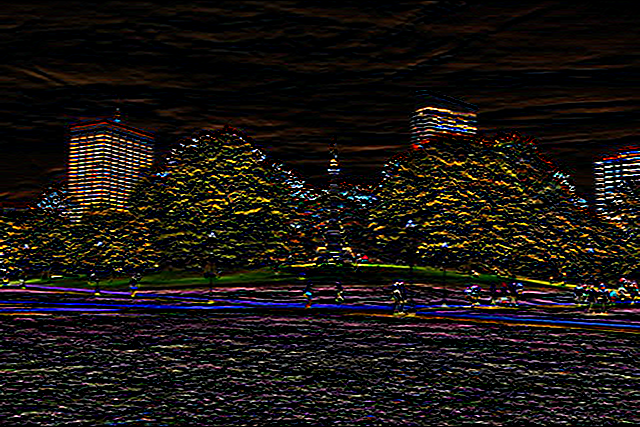
\includegraphics[width=\textwidth]{img/Horizontal.png}
          \caption{Horizontal edge detection. }
          \label{fig:horizontal_edge}
      \end{subfigure}
      \begin{subfigure}[b]{0.32\textwidth}
      \centering
          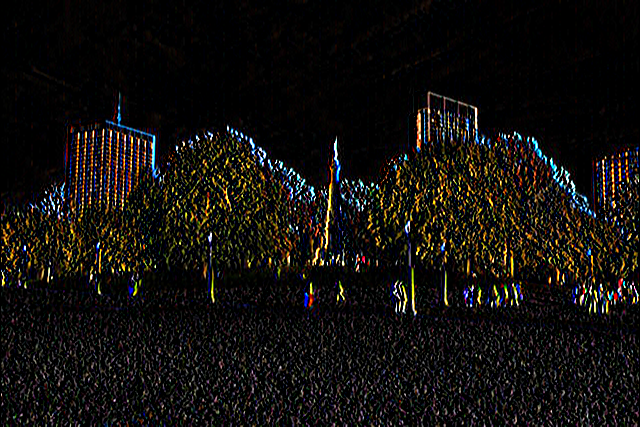
\includegraphics[width=\textwidth]{img/Vertical.png}
          \caption{Vertial edge detection. }
          \label{fig:vertical_edge}
      \end{subfigure} 

      \caption{Different convolutional kernels acting on the same image. Several useful features like edges can be detected with these simple linear maps. }
      \label{fig:feature_extraction}
    \end{figure}
  \end{example}

  We have seen in the example above that we can interpret each output channel of a convolution as a feature. That is, our original input image with $C_{in} = 3$ channels may go through a convolution that has $C_{out} = 10$ output channels, producing $10$ grayscale images. Each of these images may represent a feature that is extracted from the image through a custom kernel. When we stack convolutional layers together (with nonlinearities in between, of course), we can produce more complicated transformations that extract more abstract features. For example, while the first layer or two may extract certain edges within a dog, perhaps the fourth or fifth convolutional layer will be able to detect the presence of ears. This is a hand-wavy example, but if you actually visualize the outputs of these layers during forward prop, it is possible to see this in action.  

 
\section{Convolutional Neural Networks}  

  With convolutions in mind, we 

\subsection{Convolution Arithmetic} 

\subsection{Pooling Layers}  

  What we eventually hope for is that we can extract higher level features that can be encoded in moderate-dimensional vectors. Unfortunately, the rate at which regular convolutional filters (especially when there is padding and a stride of $1$) does not shrink the resolution of the input images at a fast enough rate. For example, having a $3 \times 3 \times 3 \times 3$ kernel with no padding on a $(3, 100, 100)$ image will decrease the dimensions to only $(3, 98, 98)$ only. Therefore, we do some very simple operations to reduce the resolution faster. 

  \begin{figure}[H]
    \centering 
    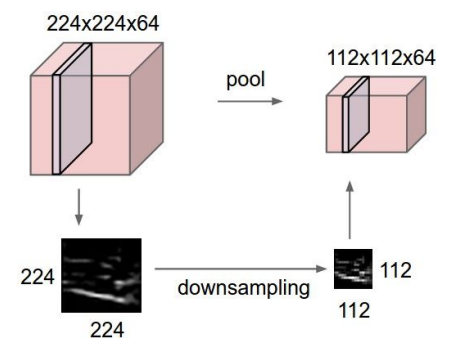
\includegraphics[scale=0.4]{img/max_pool1.png}
    \caption{} 
    \label{fig:max_pool1}
  \end{figure}

  \begin{figure}[H]
    \centering 
    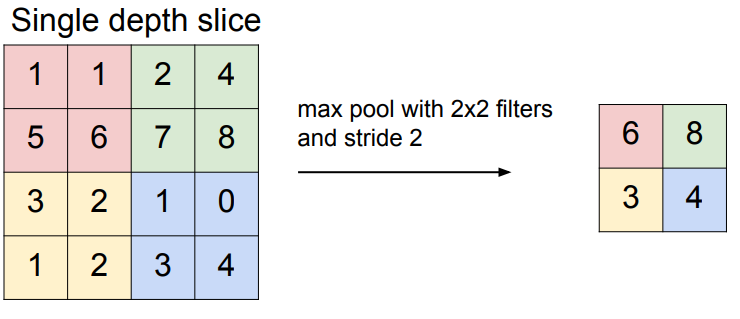
\includegraphics[scale=0.4]{img/max_pool2.png}
    \caption{} 
    \label{fig:max_pool2}
  \end{figure}

  \begin{definition}[Pooling Layers]
    A pooling layer takes in an input image of dimension $(C, H, W)$ and essentially does \textbf{downsampling} on it, involving some method of pooling local groups of pixels together into one value. There are several ways to do this: 
    \begin{enumerate}
      \item \textbf{Max Pooling} refers to dividing each channel of the image into a ``checkerboard" of $P \times P$ (where $P$ is a hyperparameter and does not necessarily have to be a square) matrices and simply choosing the maximum pixel value from it. 
      \item \textbf{Average Pooling} is the same as max pooling but we just take the average. 
    \end{enumerate}
    Clearly, these are not expensive operations and are an effective way to downsample. Therefore, the same $(3, 100, 100)$ image, after one convolutional layer followed by a pooling layer, will result in a $(3, 49, 49)$ image.  
  \end{definition}

  Ultimately, after a series of convolutions and pooling, we would want to reduce this image to a form of $(C, H, W)$, where both $H$ and $W$ are small and $C$ is large. This is because for each value of $C$, say $C = 1$, the cross section $\{(1, W, H)\}$ would encode the value of the feature identified by $C$. In fact, it could be the fact that both $H$ and $W$ are $1$, and $C = 10$. Then, we would essentially be looking at an array of $10$ numbers, which could encode the presence of some abstract features. For example, the first value $C = 1$ would encode the presence of an eye, which in the end has a value of $0.9$ (high probability), the second $C = 2$ could encode the presence of an ear, and so on. 

\subsection{Architecture} 

  Perhaps the sparsity of these maps may not allow the convolutional layers alone to extract all the features we need, so it is common to unwrap the features and then add a few fully connected layers at the end, which is much more computationally feasible now that the convolutions and pooling layers have reduced the dimensionality whilst extracting useful features with the concept of locality. This turns out to have comparable performance to regular MLPs with a fraction of the computational cost, and can easily reach $98\%$ validation accuracy on the MNIST dataset. 

  \begin{center}
    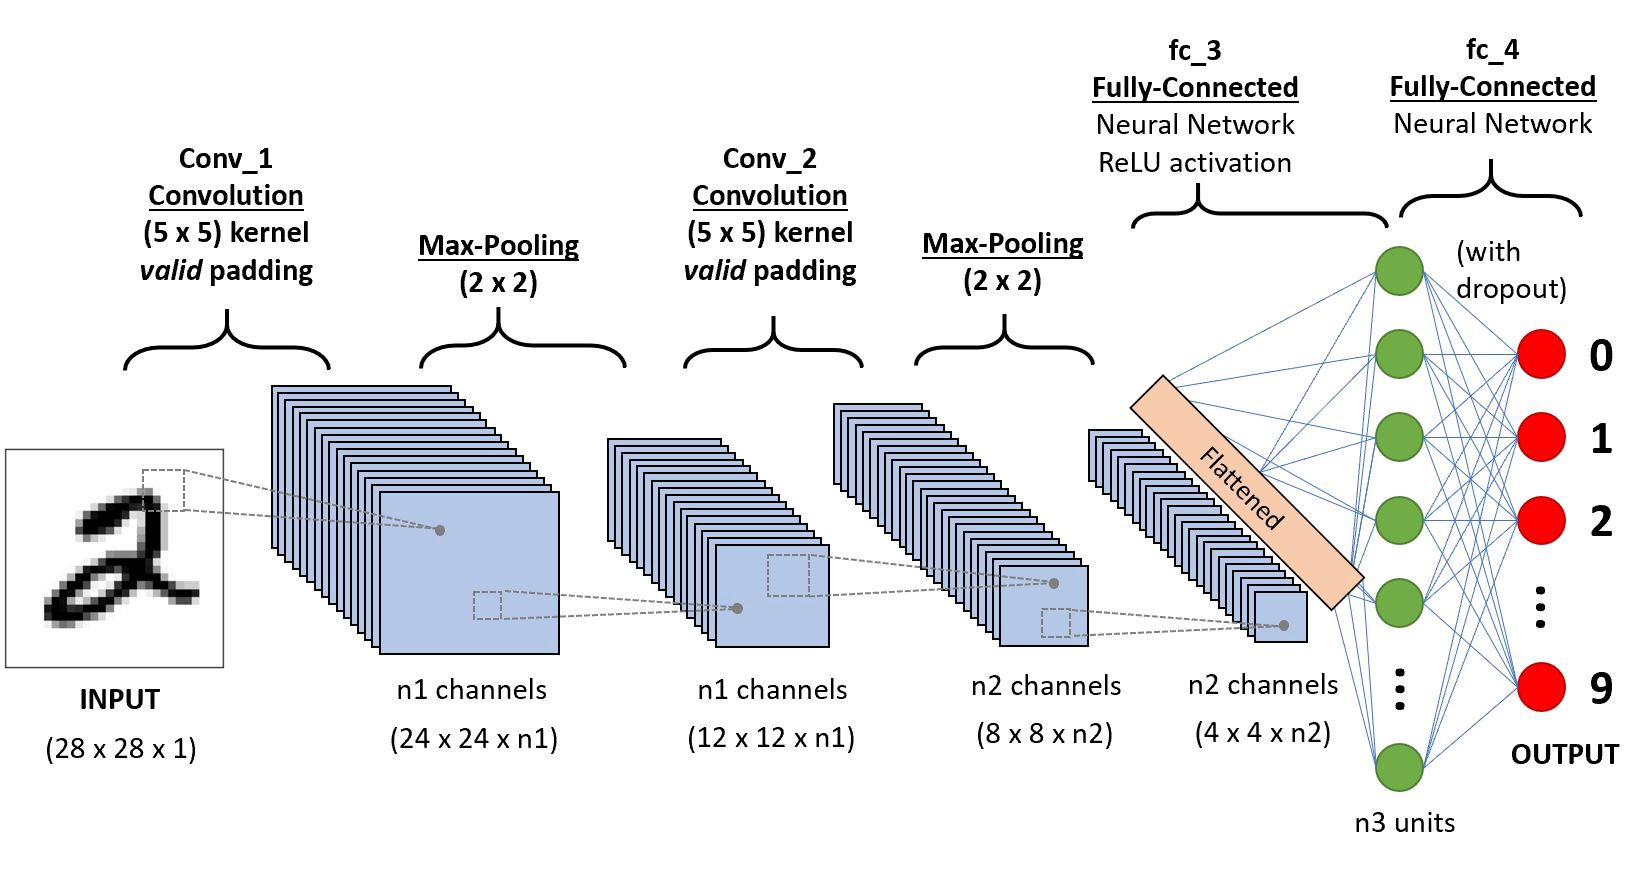
\includegraphics[scale=0.25]{img/CNN_architecture.jpeg}
  \end{center}

\subsection{Backpropagation}

  The fully connected layers are all taken care of, but now it's the convolutional layers and the pooling layers. The convolutional layers are also linear maps, so they can be treated the same way. However, the pooling layers may be nonlinear. 
  \begin{enumerate}
    \item Average pooling is linear, so no worries here. 
    \item Max pooling is not linear, but it is the next best thing: piecewise linear. 
  \end{enumerate}

 
\section{Backbone Models}

\subsection{AlexNet}

\subsection{OverFeat}

\subsection{VGG} 

 
\section{Residual Networks} 

  \begin{figure}[H]
    \centering 
    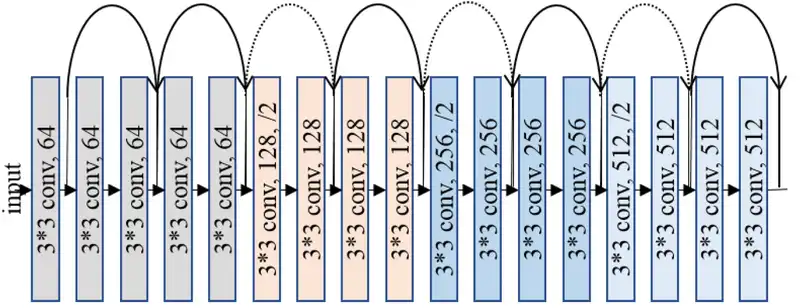
\includegraphics[scale=0.4]{img/resnet_loss.png}
    \caption{Low-dimensional visual of loss with vs without residual connections. } 
    \label{fig:resnet_loss}
  \end{figure}

  \begin{figure}[H]
    \centering 
    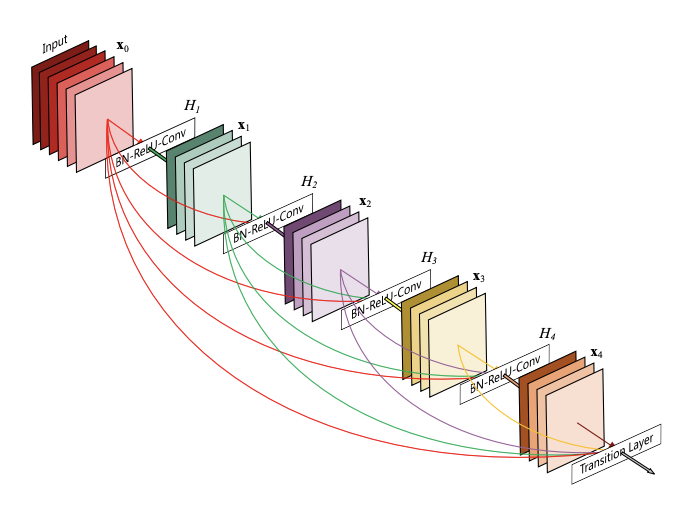
\includegraphics[scale=0.4]{img/densenet.png}
    \caption{Densenet architecture. } 
    \label{fig:densenet_architecture}
  \end{figure}

 
\section{Deconvolutions}

 
\section{Saliency Maps}

\subsection{CAM}

\subsection{Grad-CAM}

 
\section{Exercises} 

\subsection{Group Like Structures}

  \begin{exercise}[Math 401 Spring 2025 Midterm 2]
    Listed. 
    \begin{enumerate}
      \item Let $G$ be a finite group with an even number of elements. Show that $G$ contains an element of order $2$. 
      \item Prove that a group of order $10$ contains an element of order $5$. 
    \end{enumerate}
  \end{exercise}
  \begin{solution}
    Listed. 
    \begin{enumerate}
      \item We know that $e^{-1} = e$, and so remove it from $G$. Then $G$ has an odd number of elements. Now as long as $G$ is nonempty, we can remove $a, a^{-1}$, resulting in an odd cardinality. Since $G$ is finite, this must terminate, and so there must be a case where $a = a^{-1} \implies \ord(a) = 2$. 
      \item Assume that there is no element of order $5$. Then from above it must contain an element of order $2$, and let us call it $a \in G$. $\ord(e) = 1$ obviously. If any $b \in G$ had order 10, then $G = Z_{10}$, which would mean that $\ord(b^5) = 2$. Therefore every element other than the identity must have order $2$. But then given $a, b, ab \in G$, $ab \neq a, b$ since $ab = a \implies b = e$, and this is precisely the Klein 4 group. This subgroup has an order that doesn't divide 10, contradicting Lagrange's theorem. 
    \end{enumerate}
  \end{solution}

  \begin{exercise}[Shifrin 6.1.1]
    Which of the following are groups?
    \begin{enumerate}
      \item[(a)] $\{1,3,7,9\} \subset \mathbb{Z}_{10}$, with operation multiplication
      \item[(b)] $\{0,2,4,6\} \subset \mathbb{Z}_{10}$, with operation addition
      \item[(c)] $\{x \in \mathbb{Q} : 0 < x \leq 1\}$, with operation multiplication
      \item[(d)] the set of all positive irrational real numbers, with operation multiplication
      \item[(e)] the set of imaginary numbers $ix, x \in \mathbb{R}$, with operation addition
      \item[(f)] the set of complex numbers of modulus 1, with operation multiplication
      \item[(g)] $\mathbb{Z}$ with operation $a \bullet b = a + b + 1$
      \item[(h)] $\mathbb{Z}$ with operation $a \bullet b = a - b$
      \item[(i)] $\mathbb{Q} - \{1\}$ with operation $a \bullet b = a + b - ab$
    \end{enumerate}
  \end{exercise}
  \begin{solution}
    Listed. We will denote the sets in question to be $G$. 
    \begin{enumerate}
      \item[(a)] Is a group since product of 2 odds is odd, so is closed. Also we have $1$ as the identity with $3^{-1} = 7, 7^{-1} = 3, 9^{-1} = 9$. It is associative since multiplication on $\mathbb{Z}_{10}$ is associative. 
      \item[(b)] Not a group since $4 + 4 = 8 \not\in G$. 
      \item[(c)] Not a group since $1/2 \in G$ but $(1/2)^{-1} = 2 \not\in G$. 
      \item[(d)] Not a group since $\sqrt{2} \times \sqrt{2} 2  \not\in G$. 
      \item[(e)] Is a group since identity is $0 = 0i$, $ix + iy = i (x + y)$ with $x + y \in \mathbb{R}$, and $-(ix) = i (-x)$ where $-x \in \mathbb{R}$. 
      \item[(f)] Is a group since this is a representation of $O(2)$. 
      \item[(g)] Is a group since this is obviously closed under $\mathbb{Z}$ since $+_{\mathbb{Z}}$ is closed. Now assume that $i$ is the identity. Then $a \bullet i = a + i + 1 = a \implies i = -1$. Therefore $a \bullet a^{-1} = a + a^{-1} + 1 = -1 \implies a^{-1} = -a - 2$. This is associative since 
      \begin{equation}
        (a \bullet b) \bullet c = (a + b + 1) \bullet c = a + b + c + 2 = a \bullet (b + c + 1) = a \bullet (b \bullet c)
      \end{equation}
      \item[(h)] Not a group since it is not associative. Note $(a \bullet b) \bullet c = (a - b) \bullet c = a - b - c$, while $a \bullet (b \bullet c) = a \bullet (b - c) = a - b + c$. 
      \item[(i)] Is a group. We claim that it is closed. Assume not; given $a, b \neq 1$, 
        \begin{equation}
          a \bullet b = a + b - ab = 1 \implies 0 = ab - a - b + 1 = (a - 1)(b-1) 
        \end{equation}
        which means $a = 1$ or $b = 1$, which is a contradiction. As for the identity, $a \bullet i = a + i - ai = a \implies 0 = i - ai = i (1 - a) \implies i = 0$ since $a \neq 1$. We can define the inverse by solving 
        \begin{equation}
          0 = a \bullet a^{-1} = a + a^{-1} - a a^{-1} \implies a^{-1} (1 - a) = -a \implies a^{-1} = \frac{a}{a-1}
        \end{equation}
        which is well-defined since $a \neq 1$. Finally, it is associative since 
        \begin{align}
          (a \bullet b) \bullet c & = (a + b - ab) \bullet c \\
                                  & = a + b - ab + c - ac - bc - abc \\
                                  & = a + b + c - bc - ab - ac - abc \\
                                  & = a \bullet (b + c - bc) \\
                                  & = a \bullet (b \bullet c)
        \end{align}
    \end{enumerate}
  \end{solution}

  \begin{exercise}[Shifrin 6.1.10]
    \begin{enumerate}
      \item[(a)] Let $G$ be a group. Prove that $(ab)^2 = a^2b^2$ for all $a,b \in G$ if and only if $G$ is abelian.
      \item[(b)] Prove that if every element (other than the identity element) of a group $G$ has order 2, then $G$ is abelian.
    \end{enumerate}
  \end{exercise}
  \begin{solution}
    For (a), if $G$ is abelian, then 
    \begin{equation}
      (ab)^2 = (ab) (ab) = a (ba) b = a (ab) b = (aa) (bb) = a^2 b^2
    \end{equation}
    If the identity holds, then 
    \begin{equation}
      (ab)^2 = a^2 b^2 \implies (a^{-1} a) (ba) (b b^{-1}) = a^{-1} (ab)(ab) b^{-1} = a^{-1} a^2 b^2 b^{-1} \implies ba = ab
    \end{equation} 
    For (b), since we have $a^2 = e, b^2 = e$, and $(ab)^2 = e$, from (a) $G$ is abelian. 
  \end{solution}

  \begin{exercise}[Shifrin 6.1.17]
    \begin{enumerate}
      \item[(a)] A group has four elements $a$, $b$, $c$, and $d$, subject to the rules $ca = a$ and $d^2 = a$. Fill in the entire multiplication table at the left below.
      
      \begin{tabular}{c|cccc}
        $\cdot$ & $a$ & $b$ & $c$ & $d$ \\
        \hline
        $a$ & & & & \\
        $b$ & & & & \\
        $c$ & $a$ & & & \\
        $d$ & & & & $a$ \\
      \end{tabular}
      
      \item[(b)] A group has six elements $a$, $b$, $c$, $d$, $e$, and $f$, subject to the rules $ae = a$, $bd = a$, $c^2 = a$, and $df = a$. Fill in the entire multiplication table at the right above.
      
      \begin{tabular}{c|cccccc}
        $\cdot$ & $a$ & $b$ & $c$ & $d$ & $e$ & $f$ \\
        \hline
        $a$ & & & & & $a$ & \\
        $b$ & & & & $a$ & & \\
        $c$ & & & $a$ & & & \\
        $d$ & & & & & & $a$ \\
        $e$ & & & & & & \\
        $f$ & & & & & & \\
      \end{tabular}
    \end{enumerate}
  \end{exercise}
  \begin{solution}
    We can see that $ca = a \implies c = ca a^{-1} = a a^{-1} = i$, so $c$ is the identity. We can fill in the row and column of $c$. Then, we can figure out what $bd$ is. It cannot be $b$ or $d$ since $c$ is the unique identity, so it must be either $a$ or $c$. It cannot be $a$ since then $bd = a = d^2$, and so $b = d$. So it must be $c$. By the same logic we can fill out the rest of the rows and columns. 

    \begin{tabular}{c|cccc}
      $\cdot$ & $a$ & $b$ & $c$ & $d$ \\
      \hline
      $a$ & $c$ & $d$ & $a$ & $b$ \\
      $b$ & $d$ & $a$ & $b$ & $c$ \\
      $c$ & $a$ & $b$ & $c$ & $d$ \\
      $d$ & $b$ & $c$ & $d$ & $a$ \\
    \end{tabular}

    By the same logic as the previous, we can immediately see that $ae = a \implies e$ is the identity. The formal logic above can be simplified down to saying that there can be no two of the same elements in the same row or column, since if it were, then we are saying that $xy = xz \implies y = z$, which cannot be the case since $y$ and $z$ are distinct. So $fb = a$. We can also deduce that $da = ab$ and $ba = af$. At this point, we can recognize that this is the Dihedral group of order $6$, and so we fill in the rest of the multiplication table. 

    \begin{tabular}{c|cccccc}
      $\cdot$ & $a$ & $b$ & $c$ & $d$ & $e$ & $f$ \\
      \hline
      $a$ & c & f & e & b & a & d \\
      $b$ & d & e & f & a & b & c \\
      $c$ & e & d & a & f & c & b \\
      $d$ & f & c & b & e & d & a \\
      $e$ & a & b & c & d & e & f \\
      $f$ & b & a & d & c & f & e
    \end{tabular}
  \end{solution}

\subsection{Subgroups and Quotient Groups}

  \begin{exercise}[Shifrin 6.2.2]
    Prove that $\mathbb{Z}_7^{\times} \cong \mathbb{Z}_6$. (It is crucial to remember that we multiply in $\mathbb{Z}_7^{\times}$ and add in $\mathbb{Z}_6$.)
  \end{exercise}
  \begin{solution}
    Both groups are of order 6, and so $\mathbb{Z}_7^\times$---which is indeed a group (since it is the group of units of the ring $(\mathbb{Z}_7, +, \times)$)---must be isomorphic to either $\mathbb{Z}_6$ or $S_3$. However, $S_3$ is not abelian, while $\mathbb{Z}^\times_7$ is, so it must be the case that it is isomorphic to $\mathbb{Z}_6$. 
  \end{solution}

  \begin{exercise}[Shifrin 6.2.15.a/b]
    The \textbf{dihedral group} of order $2n$, denoted $\mathcal{D}_n$, is given by $\{\rho^i\psi^j : 0 \leq i < n, 0 \leq j \leq 1\}$ subject to the rules $\rho^n = e$, $\psi^2 = e$, and $\psi\rho\psi^{-1} = \rho^{-1}$.
    \begin{enumerate}
      \item Check this is really a group. That is, what is $(\rho^i\psi^j)^{-1}$, and what is the product $(\rho^i\psi^j)(\rho^k\psi^\ell)$?
      \item Check that $\mathcal{T} \cong \mathcal{D}_3$ and $S_q \cong \mathcal{D}_4$.
    \end{enumerate}
  \end{exercise}
  \begin{solution}
    We check the properties of a group. The following identity is useful: 
    \begin{equation}
      (\psi \rho \psi^{-1})^{n-i} = (\rho^{-1})^{n-i} \implies \psi \rho^{n-i} \psi^{-1} = \rho^i \implies \psi \rho^{n-i} = \rho^i \psi
    \end{equation}
    \begin{enumerate}
      \item \textit{Closure}. From simplifying according to the first two rules, we will automatically adjust the exponents to be $i, k < n$ (by subtracting out multiples of $n$) and $j \in \{0, 1\}$ (by subtracting out multiples of $2$). Going case by case, 
      \begin{enumerate}
        \item $j = 0, l = 0$. $\rho^i \rho^k = \rho^{i+k}$. 
        \item $j = 0, l = 1$. $\rho^i \rho^k \psi = \rho^{i+k} \psi$. 
        \item $j = 1, l = 0$. $\rho^i \psi \rho^k = \rho^i \rho^{n-k} \psi = \rho^{n-k+i} \psi$. 
        \item $j = 1, l = 1$. $\rho^i \psi \rho^k \psi = \rho^i \psi \psi \rho^{n-k} = \rho^i \rho^{n-k} = \rho^{n-k+i}$. 
      \end{enumerate}
      \item \textit{Identity}. The identity is $e = \rho^0 \psi^0$. We can see that $e \rho^i \psi^j = \rho^i \psi^j e = \rho^{i+0} \psi^j$. 
      \item \textit{Inverse}. We have $\psi \rho \psi^{-1} = \psi \rho \psi = \rho^{-1} \implies \psi \rho = \rho^{-1} \psi^{-1} = (\psi \rho)^{-1}$. Therefore, 
      \begin{equation}
        (\rho^i \psi^j)^{-1} = \begin{cases} 
          \rho^{n - i} & \text{ if } j = 0  \\
          \rho^{i} \psi & \text{ if } j = 1
        \end{cases}
      \end{equation}
      which are both of the correct form and therefore in $\mathcal{D}_n$. To verify, we see that $\rho^i \rho^{n-i} = \rho^n = e$, and $(\rho^i \psi) (\rho^i \psi) = \rho^i \psi \psi \rho^{n-i} = \rho^i \rho^{n-i} = e$.  
      \item \textit{Associativity}. Can also be proven tediously but problem only asked to state the product and inverse.  
    \end{enumerate} 

    For (b) for $\mathcal{T}$, we can explicitly look at the multiplication tables and see that they are isomorphic. We denote $r_1, r_2$ as the 120 and 240 degree rotations, and $f_1, f_2, f_3$ as the flips across each axis. 

    \begin{figure}[H]
      \centering
      \begin{subfigure}[b]{0.48\textwidth}
        \centering
        \begin{tabular}{c|cccccc}
          & $e$ & $\rho$ & $\rho^2$ & $\psi$ & $\rho\psi$ & $\rho^2\psi$ \\
          \hline
          $e$ & $e$ & $\rho$ & $\rho^2$ & $\psi$ & $\rho\psi$ & $\rho^2\psi$ \\
          $\rho$ & $\rho$ & $\rho^2$ & $e$ & $\rho^2\psi$ & $\psi$ & $\rho\psi$ \\
          $\rho^2$ & $\rho^2$ & $e$ & $\rho$ & $\rho\psi$ & $\rho^2\psi$ & $\psi$ \\
          $\psi$ & $\psi$ & $\rho^2\psi$ & $\rho\psi$ & $e$ & $\rho^2$ & $\rho$ \\
          $\rho\psi$ & $\rho\psi$ & $\psi$ & $\rho^2\psi$ & $\rho$ & $e$ & $\rho^2$ \\
          $\rho^2\psi$ & $\rho^2\psi$ & $\rho\psi$ & $\psi$ & $\rho^2$ & $\rho$ & $e$
        \end{tabular}
        \caption{$\mathcal{D}_3$}
      \end{subfigure}
      \hfill 
      \begin{subfigure}[b]{0.48\textwidth}
        \centering
        \begin{tabular}{c|cccccc}
          & $e$ & $r_1$ & $r_2$ & $f_1$ & $f_2$ & $f_3$ \\
          \hline
          $e$ & $e$ & $r_1$ & $r_2$ & $f_1$ & $f_2$ & $f_3$ \\
          $r_1$ & $r_1$ & $r_2$ & $e$ & $f_3$ & $f_1$ & $f_2$ \\
          $r_2$ & $r_2$ & $e$ & $r_1$ & $f_2$ & $f_3$ & $f_1$ \\
          $f_1$ & $f_1$ & $f_2$ & $f_3$ & $e$ & $r_2$ & $r_1$ \\
          $f_2$ & $f_2$ & $f_3$ & $f_1$ & $r_1$ & $e$ & $r_2$ \\
          $f_3$ & $f_3$ & $f_1$ & $f_2$ & $r_2$ & $r_1$ & $e$
        \end{tabular}
        \caption{$\mathcal{T}$}
      \end{subfigure}
    \end{figure}

    For $S_q$, it is tedious to write the full table, so we construct the isormorphisms using the generators. For $S_q$, the symmetry group of the square consists of 8 elements: the 4 rotations $r_1, r_2, r_3, r_4$ (of 90, 180, 270, and 360=0 degrees), and the flips $f_1, f_2, f_3, f_4$ (across each axis). Now we construct the function $g: \mathcal{D}_3 \rightarrow \mathcal{T}$ such that $f(\rho) = r_1$ and $f(\psi) = f_1$. Then we can see that 
    \begin{equation}
      g(\rho^4) = g(e) = e = r_1^4 = g(\rho^4), \qquad g(\psi^2) = g(e) = e = f_1^2 = g(\psi)^2
    \end{equation}
    since 90 degrees rotated 4 times is $0$ degrees, the identity, and two flips across the same axis is also the identity. Finally, we have 
    \begin{equation}
      g(\psi \rho \psi) = g(\rho^{-1}) = r_1^{-1} = r_3 = f_1 r_1 f_1 = g(\psi) g(\rho) g(\psi)
    \end{equation}
    Where $r_1^{-1} = r_3$ since a rotation of 270 after a 90 is the same as rotation by 360=0, and $r_3 = f_1 r_1 f_1$ is the change of basis symmetry observed in Shifrin Example 6.1.5. Therefore the rules match, making it a homomorphism, and since the order is the same ($\mathcal{D}_3$ has $4 \times 2 = 8$ elements from looking at the indices), this is an isomorphism. 
  \end{solution}

  \begin{exercise}[Shifrin 6.3.8]
    Let $H \subset G$ be a subgroup, and let $a \in G$ be given. Prove that $aHa^{-1} \subset G$ is a subgroup (called a \textbf{conjugate subgroup} of $H$). Prove, moreover, that it is isomorphic to $H$ (cf. Exercise 6.2.12).
  \end{exercise}
  \begin{solution}
    Let $x, y \in aHa^{-1}$. Then $x = a h_x a^{-1}, y = a h_y a^{-1}$ for some $h_x, h_y \in H$. Therefore, 
    \begin{enumerate}
      \item It is closed. $xy = (a h_x a^{-1}) (a h_y a^{-1}) = a h_x (a^{-1} a) h_y a^{-1} = a h_x h_y a^{-1} \in aHa^{-1}$ since $h_x h_y \in H$ by closure. 
      \item It has an identity since $e \in H \implies a e a^{-1} = a a^{-1} = e \in aHa^{-1}$. 
      \item It has inverses since given $x \in H$ as above with inverses $x^{-1}$, we see that $(a x a^{-1})^{-1} = (a^{-1})^{-1} x^{-1} a^{-1} = a x^{-1} a^{-1} \in a H a^{-1}$ since $x^{-1} \in H$ by $H$ being a group. 
      \item Associativity is inherited from $G$. 
    \end{enumerate} 
    It suffices to show that this is injective, since the map $\iota : H \rightarrow a H a^{-1}$ is surjective by definition. Given $x, y \in a H a^{-1}$ with $x = y$, we have $a h_x a^{-1} = a h_y a^{-1}$, and multiplying by $a$ on the right and then $a^{-1}$ on the left, we get $h_x = h_y$.
  \end{solution}

  \begin{exercise}[Shifrin 6.3.11]
    Prove that a group of order $n$ has a proper subgroup if and only if $n$ is composite.
  \end{exercise}
  \begin{solution}
    We prove bidirectionally. Call the group $G$ and subgroup $H$. 
    \begin{enumerate}
      \item $(\rightarrow)$. Assume $n$ is prime. Then by Lagrange's theorem $|H|$ must divide $n$, and so $|H| = 1$ or $n$, neither of which results in a proper subgroup. 
      \item $(\leftarrow)$. Assume $G$ has a proper subgroup $H$. Since it is proper, $|H| \neq 1, n$. Then by Lagrange's theorem, $|H|$ divides $n$, which implies that $n$ is composite. 
    \end{enumerate}
  \end{solution}

  \begin{exercise}[Shifrin 6.3.13]
    Suppose $H, K \subset G$ are subgroups of orders $5$ and $8$, respectively. Prove that $H \cap K = \{e\}$.
  \end{exercise}
  \begin{solution}
    Let us take an arbitrary element in $x \in H \cap K$ and consider the cyclic group $\langle x \rangle$. By Lagrange's Theorem, the order $|x|$ in $H$ must be either $1$ or $5$, while the order in $K$ must be $1, 2, 4, 8$. Therefore, $|x| = 1$ and so $x = e$. 
  \end{solution}

  \begin{exercise}[Shifrin 6.3.17]
    \begin{enumerate}
      \item Prove that a group $G$ of even order has an element of order $2$. (Hint: If $a \neq e$, $a$ has order $2$ if and only if $a = a^{-1}$.)
      \item Suppose $m$ is odd, $|G| = 2m$, and $G$ is abelian. Prove $G$ has precisely one element of order $2$. (Hint: If there were two, they would provide a Klein four-group.)
      \item Prove that if $G$ has exactly one element of order $2$, then it must be in the center of $G$.
    \end{enumerate}
  \end{exercise}
  \begin{solution}
    Listed. 
    \begin{enumerate}
      \item Assume the contrary and take $H = G \setminus \{e\}$. Then $|H|$ is odd, and since no element has order $2$, every element must be associated with a unique inverse $a, a^{-1}$. But this cannot happen since $|H|$ is odd. Therefore there must be at least one element of order $2$. 

      \item It has at least 1 element of order 2 from (1). Now assume that there are two, call them $a, b$. Then $ab \neq a, b$ and $ab$ also has order $2$ since $(ab)(ab) = abba = aa = e$. Therefore, calling $c = ab$, we have $ac = ca = aab = b$ and $bc = cb = abb = a$. This fully defines the multiplication table for the Klein 4 group $K$ of order $4$. Therefore, by Lagrange's theorem, we have found a subgroup $K$ and so $|K|$ must divide $G$. However, this would mean that $m$ must be even, a contradiction. Therefore there is only one such unique $a$. 

      \item Given $a \in G$ with $|a| = 2$, we wish to show that it is an element of $Z = \{ b \in G \mid bx = xb \forall x \in G\}$.\footnote{I am using the definition of center defined in Shifrin 6.3.7.} Consider $z = x^{-1} a x$. We have 
      \begin{equation}
        z^2 = (x^{-1} a x)^2 = x^{-1} a x x^{-1} a x = x^{-1} a^2 x = x^{-1} x = e
      \end{equation}
      which means that $z$ also has order $2$. But since this is unique, it must be that $z = a$. Therefore, by multiplying $x$ on the left, we get 
      \begin{equation}
        x^{-1} a x = a \implies ax = xa
      \end{equation}
    \end{enumerate}
  \end{solution}
  
  \begin{exercise}[Assigned]
    Find all group homomorphisms $\mathbb{Z}_n \to \mathbb{Z}_m$. (Your answer will depend on $n$ and $m$.) 
  \end{exercise}
  \begin{solution}
    Given a homomorphism, $f$, we must have $f(0) = 0$. Let $f(1) = k$. Note that the value of $f(1) = k$ completely determines the homomorphism since the image of every other $l \in \mathbb{Z}_n$ is defined by 
    \begin{equation}
      f(l) = f(\underbrace{1 + \ldots + 1}_{l \text{ times}}) = \underbrace{k + \ldots + k}_{l \text{ times}}
    \end{equation}
    Since the image of $f$ must be a cyclic subgroup of $\mathbb{Z}_m$, we must satisfy 
    \begin{align}
      0 = f(0) & = f(\underbrace{1 + \ldots + 1}_{n \text{ times}}) \\
               & = \underbrace{k + \ldots + k}_{n \text{ times}} 
    \end{align}
    and so $m \mid nk$. Therefore, $k$ must be a multiple of $m/\gcd(n, m)$. So all homomorphisms are determined by the set 
    \begin{equation}
      \bigg\{ k = \frac{a m}{\gcd(n, m)} \; \bigg| \; a \in \mathbb{N}, 0 \leq k \leq m-1 \bigg\}
    \end{equation}
    which we can see ranges from $0 \leq a < \gcd(n, m)$, and so the total number of homomorphisms is $\gcd(n, m)$. Note that there is always the trivial homomorphism when $a = 0$, i.e. everything maps to $0$. For example, if we have $f: \mathbb{Z}_{14} \to \mathbb{Z}_{21}$, we have $k = 0, 3, 6, 9, 12, 15, 18$. 
  \end{solution}

\subsection{Group Actions}

\subsection{Product Groups}

\subsection{Ring Like Structures}

  \begin{exercise}[Shifrin 1.2.1]
    For each of the following pairs of numbers $a$ and $b$, find $d = \gcd(a,b)$ and express $d$ in the form $ma+nb$ for suitable integers $m$ and $n$.
    \begin{enumerate}
      \item[(a)] $14, 35$
      \item[(b)] $56, 77$
      \item[(c)] $618, 336$
      \item[(d)] $2873, 6643$
      \item[(e)] $512, 360$
      \item[(f)] $4432, 1080$
    \end{enumerate}
  \end{exercise}
  \begin{solution}
    Listed. 
    \begin{enumerate}
      \item $d = 7 = (-2) \cdot 14 + (1) \cdot 35$. 
      \item $d = 7 = (-4) \cdot 56 + 3 \cdot 77$. 
      \item $d = 6 = -25 \cdot 618 + 46 \cdot 336$ 
      \item $d = 13 = 37 \cdot 2873 + (-16) \cdot 6643$. 
      \item $d = 8 = 19 \cdot 512 + (-27) \cdot 360$. 
      \item $d = 8 = 29 \cdot 4432 + (-119) \cdot 1080$. 
    \end{enumerate}
  \end{solution}

  \begin{exercise}[Shifrin 1.2.2]
    You have at your disposal arbitrarily many 4-cent stamps and 7-cent stamps. What are the postages you can pay? Show in particular that you can pay all postages greater than 17 cents.
  \end{exercise}

  \begin{exercise}[Shifrin 1.2.3]
    Prove that whenever $m \neq 0$, $\gcd(0, m) = |m|$.
  \end{exercise}

  \begin{exercise}[Shifrin 1.2.4]
    \begin{enumerate}
      \item[(a)] Prove that if $a|x$ and $b|y$, then $ab|xy$.
      \item[(b)] Prove that if $d = \gcd(a, b)$, then $\gcd(\frac{a}{d}, \frac{b}{d}) = 1$.
    \end{enumerate}
  \end{exercise}

  \begin{exercise}[Shifrin 1.2.5]
    Prove or give a counterexample: the integers $q$ and $r$ guaranteed by the division algorithm, Theorem 2.2, are unique.
  \end{exercise}

  \begin{exercise}[Shifrin 1.2.6]
     Prove or give a counterexample. Let $a, b \in \mathbb{Z}$. If there are integers $m$ and $n$ so that $d = am + bn$, then $d = \gcd(a, b)$.
  \end{exercise}

  \begin{exercise}[Shifrin 1.2.7]
    Generalize Proposition 2.5: if $\gcd(m, c) = 1$ and $m|cz$, then prove $m|z$.
  \end{exercise}
  \begin{solution}
    Let $\mathrm{gcd}(m, c) = 1$ and $m | cz$. Then there exists $a, b \in \mathbb{Z}$ such that $am + bc = 1$. Multiply both sides of the equation by $z$ to get by the distributive property 
    \begin{equation}
      (am + bc) z = amz + bcz = z
    \end{equation} 
    $m | amz$ and $m | cz \implies m | bcz$. Therefore, the sum of the two, which is equal to $z$, must be divisible by $m$. Therefore $m | z$. 
  \end{solution}

  \begin{exercise}[Shifrin 1.2.8]
    Suppose $a, b, n \in \mathbb{N}$, $\gcd(a, n) = 1$, and $\gcd(b, n) = 1$. Prove or give a counterexample: $\gcd(ab, n) = 1$.
  \end{exercise}

  \begin{exercise}[Shifrin 1.2.9]
    Prove that if $p$ is prime and $p|(a_1 a_2 \ldots a_n)$, then $p|a_j$ for some $j$, $1 \leq j \leq n$. (Hint: Use Proposition 2.5 and induction.)
  \end{exercise}

  \begin{exercise}[Shifrin 1.2.10]
    Given a positive integer $n$, find $n$ consecutive composite numbers.
  \end{exercise}

  \begin{exercise}[Shifrin 1.2.11]
    Prove that there are no integers $m, n$ so that $(\frac{m}{n})^2 = 2$. (Hint: You may start by assuming $m$ and $n$ are relatively prime. Why? Then use Exercise 1.1.3.)
  \end{exercise}

  \begin{exercise}[Shifrin 1.2.12]
    Find all rectangles whose sides have integral lengths and whose area and perimeter are equal.
  \end{exercise}

  \begin{exercise}[Shifrin 1.2.13]
    Given two nonzero integers $a, b$, in analogy with the definition of $\gcd(a, b)$, we define the \textbf{least common multiple} $\operatorname{lcm}(a, b)$ to be the positive number $\mu$ with the properties:
    \begin{enumerate}
      \item[(i)] $a|\mu$ and $b|\mu$, and
      \item[(ii)] if $s \in \mathbb{Z}$, $a|s$ and $b|s \Rightarrow \mu|s$.
    \end{enumerate}
    Prove that
    \begin{enumerate}
      \item[(a)] if $\gcd(a, b) = 1$, then $\mu = ab$. (Hint: If $\gcd(a, b) = 1$, then there are integers $m$ and $n$ so that $1 = ma + nb$; therefore, $s = mas + nbs$.)
      \item[(b)] more generally, if $\gcd(a, b) = d$, then $\mu = ab/d$.
    \end{enumerate}
  \end{exercise}
  \begin{solution}
    Listed. 
    \begin{enumerate}
      \item We can simply verify the two properties. Since $\mu = ab$, $a | \mu$ and $b | \mu$ trivially by the existence of $b$ and $a$, respectively. As for the second property, let $s \in \mathbb{Z}$ exist such that $a | s$ and $b | s$. Since $a | s$, $s = xa$ for some $x \in \mathbb{Z}$. But since $b | s$, $b | xa$. Since $\mathrm{gcd}(a, b) = 1$ by assumption, the result in [Shifrin 1.2.7] tells us that $b | x$, i.e. there exists some $k \in \mathbb{Z}$ such that $x = kb$. Therefore $s = xa = kba = kab = k \mu$. By existence of $k$, $\mu | s$, and we are done. 
      \item Given $a, b$ with $\mathrm{gcd}(a, b) = d$, there exists some $a^\prime, b^\prime \in \mathbb{Z}$ s.t. $a = da^\prime, b = db^\prime$. We claim that $\mu = ab/d \coloneqq d a^\prime b^\prime$ is the lcm.\footnote{Since division isn't generally closed in the integers, I prefer to define $ab/d$ this way.} It is clear that $a | \mu$ and $b | \mu$ by the existence of integers $b^\prime$ and $a^\prime$, respectively. To prove the second property, let $s \in \mathbb{Z}$ with $a | s$ and $b | s$. Since $a | s \iff d a^\prime | s$, there must exist some $x \in \mathbb{Z}$ s.t. $s = d a^\prime x$. But since $b | s$, this means that $d b^\prime | s \iff d b^\prime | d a^\prime x \iff b^\prime | a^\prime x$. But $\mathrm{gcd}(a^\prime, b^\prime) = 1$ which follows from the definition of gcd, and so by [Shifrin 1.2.7] it must be the case that $b^\prime | x$, i.e. there exists some $k \in \mathbb{Z}$ s.t. $x = b^\prime k$. Substituting this back we have $s = d a^\prime b^\prime k = \mu k$, and by existence of $k$ it follows that $\mu | s$. Since it satisfies these 2 properties $\mu$ is the lcm. 
    \end{enumerate}
  \end{solution} 

  \begin{exercise}[Shifrin 1.2.14]
    See Exercise 13 for the definition of $\operatorname{lcm}(a, b)$. Given prime factorizations $a = p_1^{\mu_1} \cdots p_m^{\mu_m}$ and $b = p_1^{\nu_1} \cdots p_m^{\nu_m}$, with $\mu_i, \nu_i \geq 0$, express $\gcd(a, b)$ and $\operatorname{lcm}(a, b)$ in terms of $p_1,\ldots,p_m$. Prove that your answers are correct.
  \end{exercise}

  \begin{exercise}[Shifrin 1.3.8] 
    We see that in $\bmod{10}$, 
    \begin{align}
      3^{400} \equiv 9^{200} \equiv (-1)^{200} \equiv 1^{100} \equiv 1
    \end{align} 
    so the last digit is $1$. To get the last 2 digits, we use the binomial expansion and focus on the last 2 terms. 
    \begin{equation}
      3^{400} = 9^{200} = (10 - 1)^{200} = \ldots + \binom{200}{199} 10^1 (-1)^{199} + \binom{200}{200} (-1)^{200} 
    \end{equation}
    since every combination of the form $\binom{n}{k}$ is an integer and all the other terms have a factor of $10^2$, the expansion $\bmod{100}$ becomes 
    \begin{equation}
      3^{400} \equiv \binom{200}{199} 10^1 (-1)^{199} + \binom{200}{200} (-1)^{200} = 200 \cdot 10 \cdot (-1)^{199} + 1 \equiv 1 \pmod{100}
    \end{equation}
    and so the last two digits is $01$. To get the last digit of $7^{99}$, we see that in $\bmod{10}$, 
    \begin{equation}
      7^{99} \equiv 7^{96} \cdot 7^3 \equiv (7^4)^{24} \cdot 343 \equiv 2401^{24} \cdot 343 \equiv 1^{24} \cdot 3 \equiv 3
    \end{equation}
  \end{exercise}

  \begin{exercise}[Shifrin 1.3.10]
    We must show that 
    \begin{equation}
      n \equiv 0 \pmod{13} \iff n^\prime = \sum_{i=1}^k a_i 10^{i-1} + 4a_0 \equiv 0 \pmod{13}
    \end{equation} 
    We see that $n \equiv n + 39 a_0 \equiv 0 \pmod{13}$, and 
    \begin{align}
      n + 39 a_0 & = \sum_{i=0}^k 10^i a_i + 39 a_0 \\
                 & = \sum_{i=1}^k 10^i a_i + 40 a_0 \\
                 & = 10 \bigg( \sum_{i=1}^k 10^{i-1} a_i + 4 a_0 \bigg) \\
                 & = 10 n^\prime
    \end{align} 
    and so we have $n \equiv 10 n^\prime \pmod{13}$, and so $n^\prime \equiv 0 \pmod{13} \implies n \equiv 0 \pmod{13}$. Conversely, if $n \equiv 0 \pmod{13}$, then $4n \equiv 0 \pmod{13}$, but $4n \equiv 40 n^\prime$ and so $n^\prime \equiv 40 n^\prime \equiv 4n \equiv 0 \pmod{13}$. Therefore both implications are proven. 
  \end{exercise}

  \begin{exercise}[Shifrin 1.3.12]
    Suppose that $p$ is prime. Prove that if $a^2 \equiv b^2 \pmod{p}$, then $a \equiv b \pmod{p}$ or $a \equiv -b \pmod{p}$. 
  \end{exercise}
  \begin{solution}
    We have 
    \begin{align}
      a^2 \equiv b^2 \pmod{p} & \implies a^2 - b^2 \equiv 0 \pmod{p} \\
                              & \implies (a + b) (a - b) \equiv 0 \pmod{p}
    \end{align} 
    We claim that there are no zero divisors in $\mathbb{Z}_p$. If $mn \equiv 0 \pmod{p}$, then by definition this means $p | mn$, which implies that in the integers this must mean that $p | m$ or $p | n$.\footnote{Proposition 2.5} But since $m, n \not\equiv 0$, $p \not| n$ and $p \not| m$, arriving at a contradiction. Going back to our main argument, it must be the case that $a + b \equiv 0 \implies a \equiv -b$ or $a - b \equiv 0 \implies a \equiv b$.  
  \end{solution}

  \begin{exercise}[Shifrin 1.3.15]
    Let us assume that $n = a^2 + b^2 + c^2$ for some $a, b, c \in \mathbb{Z}$. Let us consider for each integer $z$, all the possible values of $z^2 \pmod{8}$. 
    \begin{align}
      z \equiv 0 & \implies z^2 \equiv 0 \pmod{8} \\
      z \equiv 1 & \implies z^2 \equiv 1 \pmod{8} \\
      z \equiv 2 & \implies z^2 \equiv 4 \pmod{8} \\
      z \equiv 3 & \implies z^2 \equiv 1 \pmod{8} \\
      z \equiv 4 & \implies z^2 \equiv 0 \pmod{8} \\
      z \equiv 5 & \implies z^2 \equiv 1 \pmod{8} \\
      z \equiv 6 & \implies z^2 \equiv 4 \pmod{8} \\
      z \equiv 7 & \implies z^2 \equiv 1 \pmod{8} 
    \end{align}
    Therefore, $a^2 + b^2 + c^2 \pmod{8}$ can take any values of the form 
    \begin{equation}
      x + y + z \pmod{8} \text{ for } x, y, z \in \{0, 1, 4\}
    \end{equation}
    Since addition is commutative, WLOG let $x \leq y \leq z$. We can just brute force search this. 
    \begin{enumerate}
      \item If $z = 0$, then $x = y = z = 0$ and $x + y + z = 0 \not\equiv 7$. 
      \item If $z = 1$, then we see 
      \begin{align}
        0 + 0 + 1 \equiv 1 \\ 
        0 + 1 + 1 \equiv 2 \\ 
        1 + 0 + 1 \equiv 2 \\ 
        1 + 1 + 1 \equiv 3 
      \end{align}
      \item If $z = 4$, then we see that 
        \begin{align}
          0 + 0 + 4 & \equiv 4 \\
          0 + 1 + 4 & \equiv 5 \\
          0 + 4 + 4 & \equiv 0 \\
          1 + 1 + 4 & \equiv 6 \\
          1 + 4 + 4 & \equiv 1 \\
          4 + 4 + 4 & \equiv 4
        \end{align}
    \end{enumerate}
    And so $a^2 + b^2 + c^2 \not\equiv 7 \pmod{8}$ for any $a, b, c \in \mathbb{Z}$. 
  \end{exercise}

  \begin{exercise}[Shifrin 1.3.20.a/b/g]
    For (a), 
    \begin{equation}
      3x \equiv 2 \pmod{5} \implies 6x \equiv 4 \pmod{5} \implies x \equiv 4 \pmod{5} 
    \end{equation}
    For (b), 
    \begin{align}
      6x + 3 \equiv 1 \pmod{10} & \implies 6x \equiv -2 \equiv 8 \pmod{10} \\
                                & \implies 10 | (6x - 8) \\
                                & \implies 5 | (3x - 4) \\
                                & \implies 3x \equiv 4 \pmod{5} \\
                                & \implies 3x \equiv 9 \pmod{5} \\
                                & \implies x \equiv 3 \pmod{5}
    \end{align}
    For (g), 
    \begin{align}
      15x \equiv 25 \pmod{35} & \implies 35 | (15x - 25) \\
                              & \implies 7 | (3x - 5) \\
                              & \implies 3x \equiv 5 \pmod{7} \\
                              & \implies 3x \equiv 12 \pmod{7} \\ 
                              & \implies x \equiv 4 \pmod{7}
    \end{align}
  \end{exercise}

  \begin{exercise}[Shifrin 1.3.21.b/c]
    For (b), we see that $4$ and $13$ are coprime with $-3 \cdot 4 + 1 \cdot 13 = 1$. Therefore, by the Chinese remainder theorem 
    \begin{equation}
      x \equiv 1 \cdot 1 \cdot 12 + (-3) \cdot 7 \cdot 4 \pmod{52} \implies x \equiv 33 \pmod{52}
    \end{equation}
    For (c), we solve the first two congruences $x \equiv 3 \pmod{4}$ and $x \equiv 4 \pmod{5}$. $4$ and $5$ are coprime with $-1 \cdot 4 + 1 \cdot 5 = 1$. Therefore, by CRT 
    \begin{equation}
      x \equiv -1 \cdot 4 \cdot 4 + 1 \cdot 5 \cdot 3 \pmod{20} \implies x \equiv -1 \pmod{20}
    \end{equation}
    Then we solve $x \equiv -1 \pmod{20}$ with the final congruence $x \equiv 3 \pmod{7}$. We see that $20$ and $7$ are coprime with $-1 \cdot 20 + 3 \cdot 7 = 1$. Therefore by CRT 
    \begin{equation}
      x \equiv -1 \cdot 20 \cdot 3 + 3 \cdot 7 \cdot -1 \pmod{140} \implies x \equiv 59 \pmod{140}
    \end{equation}
  \end{exercise}

  \begin{exercise}[Shifrin 1.3.25]
    We prove bidirectionally. 
    \begin{enumerate}
      \item Assume a solution exists for $cx \equiv b \pmod{m}$. Then $m | (cx - b)$, which means that there exists a $y \in \mathbb{Z}$ s.t. $my = cx - b \iff b = cx - my$. Since $d = \mathrm{gcd}(c, m)$, there exists $c^\prime, m^\prime \in \mathbb{Z}$ s.t. $c = d c^\prime$ and $m = d m^\prime$. So 
      \begin{equation}
        b = cx - my = d (c^\prime x - m^\prime y) \implies d | b
      \end{equation} 

    \item Assume that $d | b$. Then there exists a $b^\prime \in \mathbb{Z}$ s.t. $b = d b^\prime$, and we have 
    \begin{align}
      cx \equiv b \pmod{m} & \iff m | (cx - b) \\
                           & \iff d m^\prime | d (c^\prime x - b^\prime) \\
                           & \iff m^\prime | (c^\prime x - b^\prime) \\
                           & \iff c^\prime x \equiv b^\prime \pmod{m^\prime} 
    \end{align}
    Since $\mathrm{gcd}(c^\prime, m^\prime) = 1$\footnote{Since $\mathrm{gcd}(c, m) = d \implies$ that there exists a $y, z \in \mathbb{Z}$ s.t. $c y + m z = d$, and dividing both sides by $d$ guarantees the existence of $y, z$ satisfying $c^\prime y + m^\prime z = 1$, meaning that $\mathrm{gcd}(c^\prime, m^\prime) = 1$.}, by Shifrin Proposition 3.5 the equation $c^\prime x \equiv b^\prime \pmod{m^\prime}$ is guaranteed to have a solution, and working backwards in the iff statements gives us the solution for $cx \equiv b \pmod{m}$. 
    \end{enumerate}

    We have proved existence of a solution in $\bmod{(m/d) = m^\prime}$. Now we show uniqueness. Assume that there are two solutions $x \equiv \alpha$, $x \equiv \beta \pmod{m^\prime}$ with $\alpha \not\equiv \beta \pmod{m^\prime}$. Then, $x$ can be written as $x = k_\alpha m^\prime + \alpha$ and $x = k_\beta m^\prime + \beta$. But we see that 
    \begin{align}
      0 = x - x & = (k_\alpha m^\prime + \alpha) - (k_\beta m^\prime + \beta) \\
                & = m^\prime (k_\alpha - k_\beta) + (\alpha - \beta) \\
                & \equiv \alpha - \beta \pmod{m^\prime}
    \end{align}
    which implies that $\alpha \equiv \beta \pmod{m^\prime}$, contradicting our assumption that they are different in modulo. Therefore the solution must be unique. 
  \end{exercise}

  \begin{exercise}[Shifrin 1.4.1]
    For $\mathbb{Z}_7$. There are no zero divisors and the units are all elements. 
    \begin{equation}
      \begin{array}{c|ccccccc}
        \times & 0 & 1 & 2 & 3 & 4 & 5 & 6 \\
        \hline
        0 & 0 & 0 & 0 & 0 & 0 & 0 & 0 \\
        1 & 0 & 1 & 2 & 3 & 4 & 5 & 6 \\
        2 & 0 & 2 & 4 & 6 & 1 & 3 & 5 \\
        3 & 0 & 3 & 6 & 2 & 5 & 1 & 4 \\
        4 & 0 & 4 & 1 & 5 & 2 & 6 & 3 \\
        5 & 0 & 5 & 3 & 1 & 6 & 4 & 2 \\
        6 & 0 & 6 & 5 & 4 & 3 & 2 & 1
      \end{array}
    \end{equation}
    For $\mathbb{Z}_8$. The zero divisors are $2, 4, 6$. The units are $1, 3, 5, 7$. 
    \begin{equation}
      \begin{array}{c|cccccccc}
        \times & 0 & 1 & 2 & 3 & 4 & 5 & 6 & 7 \\
        \hline
        0 & 0 & 0 & 0 & 0 & 0 & 0 & 0 & 0 \\
        1 & 0 & 1 & 2 & 3 & 4 & 5 & 6 & 7 \\
        2 & 0 & 2 & 4 & 6 & 0 & 2 & 4 & 6 \\
        3 & 0 & 3 & 6 & 1 & 4 & 7 & 2 & 5 \\
        4 & 0 & 4 & 0 & 4 & 0 & 4 & 0 & 4 \\
        5 & 0 & 5 & 2 & 7 & 4 & 1 & 6 & 3 \\
        6 & 0 & 6 & 4 & 2 & 0 & 6 & 4 & 2 \\
        7 & 0 & 7 & 6 & 5 & 4 & 3 & 2 & 1
      \end{array} 
    \end{equation}
    For $\mathbb{Z}_{12}$. The zero divisors are $2, 3, 4, 6, 8, 9, 10$. The units are $1, 5, 7, 11$. 
    \begin{equation}
      \begin{array}{c|cccccccccccc}
        \times & 0 & 1 & 2 & 3 & 4 & 5 & 6 & 7 & 8 & 9 & 10 & 11 \\
        \hline
        0 & 0 & 0 & 0 & 0 & 0 & 0 & 0 & 0 & 0 & 0 & 0 & 0 \\
        1 & 0 & 1 & 2 & 3 & 4 & 5 & 6 & 7 & 8 & 9 & 10 & 11 \\
        2 & 0 & 2 & 4 & 6 & 8 & 10 & 0 & 2 & 4 & 6 & 8 & 10 \\
        3 & 0 & 3 & 6 & 9 & 0 & 3 & 6 & 9 & 0 & 3 & 6 & 9 \\
        4 & 0 & 4 & 8 & 0 & 4 & 8 & 0 & 4 & 8 & 0 & 4 & 8 \\
        5 & 0 & 5 & 10 & 3 & 8 & 1 & 6 & 11 & 4 & 9 & 2 & 7 \\
        6 & 0 & 6 & 0 & 6 & 0 & 6 & 0 & 6 & 0 & 6 & 0 & 6 \\
        7 & 0 & 7 & 2 & 9 & 4 & 11 & 6 & 1 & 8 & 3 & 10 & 5 \\
        8 & 0 & 8 & 4 & 0 & 8 & 4 & 0 & 8 & 4 & 0 & 8 & 4 \\
        9 & 0 & 9 & 6 & 3 & 0 & 9 & 6 & 3 & 0 & 9 & 6 & 3 \\
        10 & 0 & 10 & 8 & 6 & 4 & 2 & 0 & 10 & 8 & 6 & 4 & 2 \\
        11 & 0 & 11 & 10 & 9 & 8 & 7 & 6 & 5 & 4 & 3 & 2 & 1
      \end{array} 
    \end{equation}
  \end{exercise}

  \begin{exercise}[Shifrin 1.4.5.a/b/c]
    \begin{enumerate}
      \item Prove that $\gcd(a, m) = 1 \iff \bar{a} \in \mathbb{Z}_m$ is a unit.
      \item Prove that if $\bar{a} \in \mathbb{Z}_m$ is a zero-divisor, then $\gcd(a, m) > 1$, and conversely, provided $m \nmid a$.
      \item Prove that every nonzero element of $\mathbb{Z}_m$ is either a unit or a zero-divisor.
      \item Prove that in any commutative ring $R$, a zero-divisor cannot be a unit, and a unit cannot be a zero-divisor. Do you think c.\ holds in general?
    \end{enumerate}
  \end{exercise}
  \begin{solution}
    For (a), 
    \begin{enumerate}
      \item $(\rightarrow)$. If $\mathrm{gcd}(a, m) = 1$, then there exists $x, y \in \mathbb{Z}$ such that $ax + my = 1$. Taking the modulo on both sides gives $ax \equiv 1 \pmod{m}$, and therefore we have established the existence of $x \in \mathbb{Z}$, which implies the existence of $\bar{x} \in \mathbb{Z}_m$. 

      \item $(\leftarrow)$. If we have $a \in \mathbb{Z}$ and $\bar{a}$ is a unit, then there exists a $\bar{x} \in \mathbb{Z}_m$ s.t. $\bar{a} \bar{x} = \bar{1} \iff ax \equiv 1 \pmod{m}$, which means that $m | (1 - ax)$. So there exists an integer $y \in \mathbb{Z}$ s.t. $my = 1 - ax \iff ax + my = 1$. By Shifrin corollary 2.4 $a, m$ must be coprime. 
    \end{enumerate}

    For (b), 
    \begin{enumerate}
      \item ($\rightarrow$) Let $\bar{a} \in \mathbb{Z}_m$ be a zero-divisor. Then there exists $\bar{x} \neq \bar{0}$ in $\mathbb{Z}_m$ such that $\bar{a}\bar{x} = \bar{0}$. This means: $ax \equiv 0 \pmod{m}$, so $m \mid ax$, and  $m \nmid x$ (since $\bar{x} \neq \bar{0}$). Since $m \mid ax$ but $m \nmid x$, some prime factor of $m$ must divide $a$. This prime factor is then a common divisor of $a$ and $m$ greater than 1, so $\gcd(a,m) > 1$.

      \item ($\leftarrow$) Let $a \in \mathbb{Z}$, $m \in \mathbb{N}$ where $\gcd(a, m) = d > 1$ and $m \nmid a$. Then $a = a'd$ and $m = m'd$ for some $a', m' \in \mathbb{Z}$. Therefore, 
      \begin{equation}
        \bar{a} \bar{m'} = \overline{am'} = \overline{a'd m'} = \overline{a'm} = \bar{0}
      \end{equation}
      Also since $m \nmid a$, we have $\bar{a} \neq \bar{0}$, and since $m = m'd$, we have $m \nmid m'$ (since $m \nmid a \implies d \neq m$), so $\bar{m'} \neq \bar{0}$. Therefore $\bar{a}$ is a zero-divisor in $\mathbb{Z}_m$.
    \end{enumerate}

    For (c), let $a \in \mathbb{Z}_m$ be a nonzero element. Then it must be the case that $\mathrm{gcd}(a, m) = 1$ or $\mathrm{gcd}(a, m)  > 1$. In the former case, $a$ is a unit by (a), and in the latter case, $a \not\equiv 0 \implies m \nmid a$\footnote{By contrapositive $m \mid a \implies a \equiv 0 \pmod{m}$ is trivial.}, and so by (b) $a$ is a zero divisor. 
  \end{solution}

  \begin{exercise}[Shifrin 1.4.6.b/c/d]
    Prove that in any ring $R$:
    \begin{enumerate}
      \item $0 \cdot a = 0$ for all $a \in R$ (cf.\ Lemma 1.1);
      \item $(-1)a = -a$ for all $a \in R$ (cf.\ Lemma 1.2);
      \item $(-a)(-b) = ab$ for all $a,b \in R$;
      \item the multiplicative identity $1 \in R$ is unique.
    \end{enumerate}
  \end{exercise}
  \begin{solution} 
    For (a), note that $0 a = (0 + 0) \cdot a = 0a + 0a$ and by subtracting $0a$ from both sides, we have $0 = 0a$. Similarly, $a0 = a (0 + 0) = a0 + a0 \implies 0 = a0$. 
    For (b), 
    \begin{align}
      a + (-1) \cdot a & = 1 \cdot a + (-1) \cdot a && \tag{definition of $1$} \\
                       & = (1 + -1) \cdot a && \tag{left distributivity} \\
                       & = 0 \cdot a && \tag{definition of add inverse}\\
                       & = 0 && \tag{From (a)}
    \end{align}
    For (c), note that by right distributivity, 
    \begin{align}
      (-1) \cdot a + a & = (-1) \cdot a + 1 \cdot a && \tag{definition of $1$} \\
                       & = (-1 + 1) \cdot a && \tag{right distributivity} \\
                       & = a \cdot 0 && \tag{definition of add inverse}\\
                       & = 0 && \tag{From (a)}
    \end{align}
    Therefore, 
    \begin{align}
      (-a)(-b) & = (-1 \cdot a) (-1 \cdot b) && \tag{from (b)}\\
               & = -1 \cdot (a \cdot -1) \cdot b && \tag{associativity} \\
               & = -1 \cdot -a \cdot b && \tag{from (b)} \\
               & = -1 \cdot -1 \cdot a \cdot b && \tag{from (b)} \\
               & = (-1 \cdot -1) \cdot ab && \tag{associativity} \\
               & = 1ab && \tag{shown below}\\
               & = ab && \tag{definition of identity}
    \end{align} 
    where $(-1)(-1) = 1$ since by (b), $(-1)(-1) = -(-1)$. We know that $-(-1)$ is an additive inverse for $-1$ and so is $1$. Since the multiplicative identity is unique in a ring, $-(-1) = 1$.  We show uniqueness for (d). Let us have $1 \neq 1^\prime$. Then by definition of identity, 
    \begin{equation}
      1 = 1 1^\prime = 1^\prime 1 = 1^\prime
    \end{equation}
    which is a contradiction. 
  \end{solution}

  \begin{exercise}[Shifrin 1.4.10]
    \begin{enumerate}
      \item Prove that the multiplicative inverse of a unit $a$ in a ring $R$ is unique. That is, if $ab = ba = 1$ and $ac = ca = 1$, then $b = c$. (You will need to use associativity of multiplication in $R$.)
      
      \item Indeed, more is true. If $a \in R$ and there exist $b,c \in R$ so that $ab = 1$ and $ca = 1$, prove that $b = c$ and thus that $a$ is a unit.
    \end{enumerate}
  \end{exercise}
  \begin{solution}
    For (a), we see that 
    \begin{equation}
      c = 1c = (ab)c = (ba)c = b(ac) = b(ca) = b1 = b
    \end{equation} 
    For (b), we have  
    \begin{equation}
      b = 1b = (ca)b = c(ab) = c1 = c
    \end{equation}
  \end{solution}

  \begin{exercise}[Shifrin 1.4.13]
    Let $p$ be a prime number. Use the fact that $\mathbb{Z}_p$ is a field to prove that $(p-1)! \equiv -1 \pmod{p}$. (Hint: Pair elements of $\mathbb{Z}_p$ with their multiplicative inverses; cf. Exercise 1.3.12.). 
  \end{exercise}
  \begin{solution}
    For $p = 2$, the result is trivial. Now let $p > 2$ be a prime. Then since $\mathbb{F}$ is a field, every element $a \in \mathbb{F}$ contains a multiplicative inverse $a^{-1}$. We claim that the only values for which $a = a^{-1}$ is $1, p-1$. Assume that $a = a^{-1}$. Then 
    \begin{equation}
      a^2 = 1 \implies p|(a^2 - 1) \implies p | (a+1)(a-1)
    \end{equation}
    and since $p$ is prime, it must be the case that $p|a+1 \iff a \equiv -1 \pmod{p}$ or $p|a-1 \iff a \equiv 1 \pmod{p}$. Therefore, we are left to consider the $(p-3)$ elements: $2, \ldots, p-2$. Since inverses are unique and the inverses of inverses is the original element, we can partition these $p-2$ elements into $(p-3)/2$ pairs.\footnote{Since $p \neq 2$, $p$ is odd and therefore $p-3$ is even.} Let's call the set of pairs $K = \{(a, b)\}$ where $b = a^{-1}$. Therefore, by commutativity and associativity we have 
    \begin{equation}
      (p-1)! \equiv (1)(p-1) \prod_{(a, b) \in K} ab \equiv -1 \cdot \prod_{(a, b) \in K} 1 \equiv -1 \pmod{p}. 
    \end{equation}
  \end{solution} 

  \begin{exercise}[Shifrin 2.3.2.a/b/c]
    Recall that the conjugate of the complex number $z = a + bi$ is defined to be $\bar{z} = a - bi$. Prove the following properties of the conjugate:
    \begin{enumerate}
      \item $\overline{z + w} = \bar{z} + \bar{w}$
      \item $\overline{zw} = \bar{z}\bar{w}$
      \item $\bar{z} = z \iff z \in \mathbb{R}$ and $\bar{z} = -z \iff iz \in \mathbb{R}$
      \item If $z = r(\cos\theta + i\sin\theta)$, then $\bar{z} = r(\cos\theta - i\sin\theta)$
    \end{enumerate}
  \end{exercise}
  \begin{solution}
    Let $z = a + bi, w = c + di$. For (a), 
    \begin{equation}
      \overline{z + w} = \overline{(a + c) + (b + d)i} = (a + c) - (b + d)i = a + c - bi - di = (a - bi) + (c - di) = \overline{z} + \overline{w}
    \end{equation} 
    For (b), 
    \begin{equation}
      \overline{zw} = \overline{(ac - bd) + (ad + bc)i} = (ac - bd) - (ad + bc)i = ac - bd - adi - bci = (a - bi)(c - di) = \bar{z}\bar{w}
    \end{equation}
    For (c), consider 
    \begin{align}
      \overline{z} = z & \iff a + bi = a - bi \\
                       & \iff bi = -bi \\
                       & \iff 2bi = 0 \\
                       & \iff b = 0 && \tag{field has no 0 divisors}
    \end{align}
    Therefore, $z = a \in \mathbb{R}$. 
    \begin{align}
      \overline{z} = -z & \iff a - bi = -a - bi \\
                        & \iff a = -a \\
                        & \iff 2a = 0 \\
                        & \iff a = 0 && \tag{field has no 0 divisors.}
    \end{align}
    Therefore, $z = bi \implies iz = -b \in \mathbb{R}$. 
  \end{solution}

  \begin{exercise}[Shifrin 2.3.3.a/b/c]
    Recall that the modulus of the complex number $z = a + bi$ is defined to be $|z| = \sqrt{a^2 + b^2}$. Prove the following properties of the modulus:
    \begin{enumerate}
      \item $|zw| = |z||w|$
      \item $|\bar{z}| = |z|$
      \item $|z|^2 = z\bar{z}$
      \item $|z + w| \leq |z| + |w|$ (This is called the triangle inequality; why?)
    \end{enumerate}
  \end{exercise}
  \begin{solution}
    Let $z = a + bi$ and $w = c + di$. For (a),
    \begin{align*}
      |zw| &= |(ac - bd) + (ad + bc)i| \\
      &= \sqrt{(ac - bd)^2 + (ad + bc)^2} \\
      &= \sqrt{a^2c^2 - 2abcd + b^2d^2 + a^2d^2 + 2abcd + b^2c^2} \\
      &= \sqrt{(a^2 + b^2)(c^2 + d^2)} \\
      &= \sqrt{a^2 + b^2}\sqrt{c^2 + d^2} \\
      &= |z||w|
    \end{align*}

    For (b), if $z = a + bi$, then $\bar{z} = a - bi$, so:
    \begin{equation}
      |\bar{z}| = \sqrt{a^2 + (-b)^2} = \sqrt{a^2 + b^2} = |z|
    \end{equation}

    For (c),
    \begin{align*}
      z\bar{z} &= (a + bi)(a - bi) \\
      &= a^2 + b^2 \\
      &= |z|^2
    \end{align*}
  \end{solution}

  \begin{exercise}[Shifrin 3.1.2.c/d]
    Find the greatest common divisors $d(x)$ of the following polynomials $f(x), g(x) \in F[x]$, and express $d(x)$ as $s(x)f(x) + t(x)g(x)$ for appropriate $s(x), t(x) \in F[x]$:
    \begin{enumerate}
      \item $f(x) = x^3 - 1$, $g(x) = x^4 + x^3 - x^2 - 2x - 2$, $F = \mathbb{Q}$
      \item $f(x) = x^2 + (1 - \sqrt{2})x - \sqrt{2}$, $g(x) = x^2 - 2$, $F = \mathbb{R}$
      \item $f(x) = x^2 + 1$, $g(x) = x^2 - i + 2$, $F = \mathbb{C}$
      \item $f(x) = x^2 + 2x + 2$, $g(x) = x^2 + 1$, $F = \mathbb{Q}$
      \item $f(x) = x^2 + 2x + 2$, $g(x) = x^2 + 1$, $F = \mathbb{C}$
    \end{enumerate}
  \end{exercise}
  \begin{solution}
    For (c), the gcd is $1$, with 
    \begin{equation} 
      -\frac{1}{1 - i} (x^2 + 1) + \frac{1}{1 - i} (x^2 - i + 2) = \frac{1}{1-i} (x^2 - i + 2 - x^2 - 1) = \frac{1}{1-i} (1 - i) = 1
    \end{equation}
    where $1/(1-i) = (1 + i)/2$. For (d), the gcd is $1$, with 
    \begin{align}
      \frac{1}{5} (2x + 3) (x^2 + 1) & + \frac{1}{5} (1 - 2x) (x^2 + 2x + 2) \\
                                          & = \frac{1}{5} (2x^3 + 3x^2 + 2x + 3) + \frac{1}{5} (-2x^3 - 3x^2 - 2x + 2) = 1
    \end{align}
  \end{solution}

  \begin{exercise}[Shifrin 3.1.6]
    Prove that if $F$ is a field, $f(x) \in F[x]$, and $\mathrm{deg}(f(x)) = n$, then $f(x)$ has at most $n$ roots in $F$. 
  \end{exercise}
  \begin{solution}
    We start when $n=1$. Then $f(x) = mx + b$ and we claim that the only root is $x = -b/m$ since we can solve for $0 = mx + b$ with the field operations, which leads to a unique solution. This implies by corr 1.5 that $(x + b/m)$ is the only factor of $f$. Now suppose this holds true for some degree $n-1$ and let us have a degree $n$ polynomial $f$. Assume that some $c$ is a root of $f$ (if there exists no $c$, then we are trivially done), which means $(x - c)$ is a factor of $f$, and we can write 
    \begin{equation}
      f(x) = (x - c) \, g(x)
    \end{equation}
    for some polynomial $g(x)$ of degree $n-1$. By our inductive hypothesis, $g(x)$ must have at most $n-1$ roots, and so $f$ has at most $n$ roots. 
  \end{solution}

  \begin{exercise}[Shifrin 3.1.8]
    Let $F$ be a field. Prove that if $f(x) \in F[x]$ is a polynomial of degree $2$ or $3$, then $f(x)$ is irreducible in $F[x]$ if and only if $f(x)$ has no root in $F$.
  \end{exercise}
  \begin{solution}
    We prove bidirectionally. 
    \begin{enumerate}
      \item $(\rightarrow)$. Let $f$ be irreducible. Then it cannot be factored into polynomials $p(x) q(x)$ where $\mathrm{deg}(p) + \mathrm{deg}(q) = n$. Note that two positive integers adding up to $2$ or $3$ means that at least one of the integers must be $1$, by the pigeonhole principle. This means that $f$ irreducible is equivalent to saying that $f$ does not have linear factors of form $(x-c)$, which by corollary 1.5 implies that there exists no root $c$ for $f(x)$. 
      \item $(\leftarrow)$. Let $f$ have no root in $F$. Then by corollary 1.5 there exists no linear factors $(x-c)$. By the same pigeonhole principle argument, we know that having a linear factor for degree 2 or 3 polynomials is equivalent to having (general) factors, and so $f$ has no factors. Therefore $f$ is irreducible. 
    \end{enumerate}
  \end{solution}

  \begin{exercise}[Shifrin 3.1.13]
    List all the irreducible polynomials in $\mathbb{Z}_2[x]$ of degree $\leq 4$. Factor $f(x) = x^7 + 1$ as a product of irreducible polynomials in $\mathbb{Z}_2[x]$.
  \end{exercise}
  \begin{solution}
    Listed by degree. 
    \begin{enumerate}
      \item $1$: $x, x + 1$. 
      \item $2$: $x^2 + x + 1$. 
      \item $3$: $x^3 + x^2 + 1, x^3 + x + 1$. 
      \item $4$: $x^4 + x + 1, x^4 + x^3 + 1, x^4 + x^3 + x^2 + x + 1$. 
    \end{enumerate}
    We have 
    \begin{align}
      x^7 + 1 & = (x + 1)(x^6 + x^5 + x^4 + x^3 + x^2 + x + 1) \\
              & = (x + 1) (x^3 + x + 1) (x^3 + x^2 + 1)
    \end{align}
  \end{solution}

  \begin{exercise}[Shifrin 3.2.2.b/c]
    Prove that
    \begin{enumerate}
      \item $\mathbb{Q}[\sqrt{2}, i] = \mathbb{Q}[\sqrt{2} + i]$, but $\mathbb{Q}[\sqrt{2}i] \subsetneq \mathbb{Q}[\sqrt{2}, i]$
      \item $\mathbb{Q}[\sqrt{2}, \sqrt{3}] = \mathbb{Q}[\sqrt{2} + \sqrt{3}]$, but $\mathbb{Q}[\sqrt{6}] \subsetneq \mathbb{Q}[\sqrt{2}, \sqrt{3}]$
      \item $\mathbb{Q}[\sqrt[3]{2} + i] = \mathbb{Q}[\sqrt[3]{2}, i]$; what about $\mathbb{Q}[\sqrt[3]{2}i] \subset \mathbb{Q}[\sqrt[3]{2}, i]$?
    \end{enumerate}
  \end{exercise}
  \begin{solution}[Shifrin 3.2.2.b]
    From Shifrin, I use the fact that $\mathbb{Q}[\sqrt{2}] = \{ a + b \sqrt{2} \mid a, b \in \mathbb{Q}\}$, and the same proof immediately shows that $\mathbb{Q}[\sqrt{3}] = \{ a + b \sqrt{3} \mid a, b \in \mathbb{Q}\}$ along with that for $\mathbb{Q}[\sqrt{6}]$. As for $\mathbb{Q}[\sqrt{2}, \sqrt{3}]$, I also follow the same logic to show 
    \begin{align}
      \mathbb{Q}[\sqrt{2}, \sqrt{3}] & = \mathbb{Q}[\sqrt{2}][\sqrt{3}] \\
                                     & = \{\alpha + \beta \sqrt{3} \mid a, b \in \mathbb{Q}[\sqrt{2}]\} \\
                                     & = \{ (a + b\sqrt{2}) + (c + d \sqrt{2}) \sqrt{3} \mid a, b, c, d \in \mathbb{Q} \} \\
                                     & = \{ a + b\sqrt{2} + c \sqrt{3} + d \sqrt{6} \mid a, b, c, d \in \mathbb{Q} \} 
    \end{align}
    Where $\sqrt{2} \times \sqrt{3} = \sqrt{2 \times 3} = \sqrt{6}$ follows from the definition of $n$th roots plus associativity on the reals. For (b), we prove bidirectionally.
    \begin{enumerate}
      \item $\mathbb{Q}[ \sqrt{2} + \sqrt{3}] \subset \mathbb{Q}[\sqrt{2}, \sqrt{3}]$. Consider $y \in \mathbb{Q}[\sqrt{2} + \sqrt{3}]$. Then there exists $p \in \mathbb{Q}[x]$ s.t. 
      \begin{equation}
        y = p(\sqrt{2} + \sqrt{3}) = a_n (\sqrt{2} + \sqrt{3})^n + \ldots + a_1 (\sqrt{2} + \sqrt{3}) + a_0
      \end{equation}
      where the terms can be expanded an rearranged to the form $a + b \sqrt{2} + c \sqrt{3} + d \sqrt{6} \in \mathbb{Q}[\sqrt{2}, \sqrt{3}]$. 

    \item $\mathbb{Q}[\sqrt{2}, \sqrt{3}] \subset \mathbb{Q}[ \sqrt{2} + \sqrt{3}]$. Consider $\sqrt{2} + \sqrt{3} \in \mathbb{Q}[\sqrt{2} + \sqrt{3}]$. Since it is a field and $\sqrt{2} + \sqrt{3}$ is a unit, by rationalizing the denominator, we can get 
      \begin{equation}
        (\sqrt{2} + \sqrt{3})^{-1} = \frac{\sqrt{2} - \sqrt{3}}{2 - 3} = \sqrt{3} - \sqrt{2} \in \mathbb{Q}[\sqrt{2} + \sqrt{3}]
      \end{equation}
      Therefore by adding and subtracting the two elements, we have $\sqrt{2}, \sqrt{3} \in \mathbb{Q}[\sqrt{2} + \sqrt{3}] \implies \sqrt{6} \in \mathbb{Q}[\sqrt{2} + \sqrt{3}]$. Since $\mathbb{Q} \subset \mathbb{Q}[\sqrt{2} + \sqrt{3}]$, from the ring properties all elements of the form $a + b \sqrt{2} + c \sqrt{3} + d \sqrt{6} \in \mathbb{Q}[\sqrt{2} + \sqrt{3}]$. 
    \end{enumerate}

    For the second part, I claim that $\sqrt{2} \not\in \mathbb{Q}[\sqrt{6}]$. Assuming it is, we have $\sqrt{2} = a + b \sqrt{6} \implies 2 = a^2 + 6b^2 + 2ab \sqrt{6}$. So $a = 0$ or $b = 0$. If $a = 0$, then $b^2 = 1/3 \implies b = 1/\sqrt{3}$ which contradicts that $b$ is rational. If $b = 0$, then $a^2 = 2 \implies a = \sqrt{2}$ which contradicts that $a$ is rational. 
  \end{solution}

  \begin{solution}[Shifrin 3.2.2.c]
    Note that $\mathbb{Q}[\sqrt[3]{2}] = \{a + b \sqrt[3]{2} + c \sqrt[3]{4}\}$, and so 
    \begin{align}
      \mathbb{Q}[\sqrt[3]{2}, i] & = \mathbb{Q}[\sqrt[3]{2}][i] \\
                                 & = \{\alpha + \beta i \mid \alpha, \beta \in \mathbb{Q}[\sqrt[3]{2}]\} \\
                                 & = \{ (a + b \sqrt[3]{2} + c \sqrt[3]{4}) + (d + e \sqrt[3]{2} + f \sqrt[3]{4}) i \mid a, b, c, d, e, f \in \mathbb{Q}\} \\
                                 & = \{ a + b \sqrt[3]{2} + c \sqrt[3]{4} + d i + e \sqrt[3]{2} i + f \sqrt[3]{4} i \mid a, b, c, d, e, f \in \mathbb{Q}\}
    \end{align}
    We prove bidirectionally. 
    \begin{enumerate}
      \item $\mathbb{Q}[\sqrt[3]{2} + i] \subset \mathbb{Q}[\sqrt[3]{2}, i]$. Consider $y \in \mathbb{Q}[\sqrt[3]{2} + i]$. Then there exists a $p \in \mathbb{Q}[x]$ s.t. 
      \begin{equation}
        y = p(\sqrt[3]{2} + i) = a_n (\sqrt[3]{2} + i)^n + \ldots + a_1 (\sqrt[3]{2} + i) + a_0
      \end{equation}
      Then we can expand and rearrange the terms to be of the form 
      \begin{equation}
        a + b \sqrt[3]{2} + c \sqrt[3]{4} + d i + e i \sqrt[3]{2} + f i \sqrt[3]{4} \in \mathbb{Q}[\sqrt[3]{2}, i]
      \end{equation}

      \item $\mathbb{Q}[\sqrt[3]{2}, i] \subset \mathbb{Q}[\sqrt[3]{2} + i]$. Consider $\alpha = \sqrt[3]{2} + i \in \mathbb{Q}[\sqrt[3]{2} + i]$. Then $(\alpha - i)^3 = 2$. Therefore 
      \begin{align}
        \alpha^3 - 3 \alpha^2 i - 3 \alpha + i = 2 & \implies i(1 - 3 \alpha^2) = 2 + 3 \alpha - \alpha^3 \\ 
                                                   & \implies i = \frac{2 + 3 \alpha - \alpha^3}{1 - 3 \alpha^2} \in \mathbb{Q}[\sqrt[3]{2} + i]
      \end{align}
      Therefore $\sqrt[3]{2} = \alpha - i \in \mathbb{Q}[\sqrt[3]{2} + i]$, which allows us add all combinations $\{1, \sqrt[3]{2}, \sqrt[3]{4}, i, \sqrt[3]{2} i, \sqrt[3]{4} i\}$ into our basis. 
    \end{enumerate}
  \end{solution}

  \begin{exercise}[Shifrin 3.2.6.b/c/d/g]
    Suppose $\alpha \in \mathbb{C}$ is a root of the given irreducible polynomial $f(x) \in \mathbb{Q}[x]$. Find the multiplicative inverse of $\beta \in \mathbb{Q}[\alpha]$.
    \begin{enumerate}
      \item $f(x) = x^2 + 3x - 3$, $\beta = \alpha - 1$ 
      \item $f(x) = x^3 + x^2 - 2x - 1$, $\beta = \alpha + 1$
      \item $f(x) = x^3 + x^2 + 2x + 1$, $\beta = \alpha^2 + 1$
      \item $f(x) = x^3 - 2$, $\beta = \alpha + 1$
      \item $f(x) = x^3 + x^2 - x + 1$, $\beta = \alpha + 2$
      \item $f(x) = x^3 - 2$, $\beta = r + s\alpha + t\alpha^2$
      \item $f(x) = x^4 + x^2 - 1$, $\beta = \alpha^3 + \alpha - 1$
    \end{enumerate}
  \end{exercise}
  \begin{solution}
    For (b), using the Euclidean algorithm gives 
    \begin{equation}
      (1) (x^3 + x^2 - 2x - 1) + (-x^2 + 2) (x + 1) = 1 
    \end{equation}
    and substituting the root $\alpha$ gives $(-\alpha^2 + 2)(\alpha + 1) = 1$. So we have $\beta^{-1} = -\alpha^2 + 2$.  
    For (c), doing the same thing gives 
    \begin{equation}
      (-x) (x^3 + x^2 + 2x + 1) + (x^2 + x + 1)(x^2 + 1) = 1
    \end{equation}
    and substituting $\alpha$ gives $(\alpha^2 + \alpha + 1)(\alpha^2 + 1) = 1$, so $\beta^{-1} = \alpha^2 + \alpha + 1$. 
    For (d), we have 
    \begin{equation}
      (-\frac{1}{3}) (x^3 - 2) + (\frac{1}{3} x^2 - \frac{1}{3} x + \frac{1}{3}) (x + 1) = 1 
    \end{equation}
    and so substituting $\alpha$ gives $(\frac{1}{3} \alpha^2 - \frac{1}{3} \alpha + \frac{1}{3}) (\alpha + 1) = 1$, so $\beta^{-1} = \frac{1}{3} \alpha^2 - \frac{1}{3} \alpha + \frac{1}{3}$. For (g), we have 
    \begin{equation}
      (-x^2 - x - 2) (x^4 + x^2 - 1) + (x^3 + x^2 + 2x + 1) (x^3 + x - 1) = 1
    \end{equation}
    and so substituting $\alpha$ gives $(\alpha^3 + \alpha^2 + 2\alpha + 1) (\alpha^3 + \alpha - 1) = 1$, and so $\beta^{-1} = \alpha^3 + \alpha^2 + 2\alpha + 1$. 
  \end{solution}

  \begin{exercise}[Shifrin 3.2.7]
    Let $f(x) \in \mathbb{R}[x]$.
    \begin{enumerate}
      \item Prove that the complex roots of $f(x)$ come in ``conjugate pairs''; i.e., $\alpha \in \mathbb{C}$ is a root of $f(x)$ if and only if $\overline{\alpha}$ is also a root.
      \item Prove that the only irreducible polynomials in $\mathbb{R}[x]$ are linear polynomials and quadratic polynomials $ax^2 + bx + c$ with $b^2 - 4ac < 0$.
    \end{enumerate}
  \end{exercise}
  \begin{solution}
    Listed. 
    \begin{enumerate}
      \item If $\alpha \in \mathbb{C}$ is a root of $f$, then 
      \begin{equation}
        0 = f(\alpha) = a_n \alpha^n + \ldots + a_1 \alpha + a_0
      \end{equation}
      for $a_i \in \mathbb{R}$. Since 
      \begin{align}
        0 = \overline{0} & = \overline{f(\alpha)} \\
                         & = \overline{a_n \alpha^n + \ldots + a_1 \alpha + a_0} \\
                         & = \overline{a_n} \overline{\alpha^n} + \ldots + \overline{a_1} \overline{\alpha} + \overline{a_0} \\
                         & = a_n \overline{\alpha}^n + \ldots + a_1 \overline{\alpha} + a_0 \\
                         & = p(\overline{\alpha})
      \end{align} 
      we can see that $\overline{\alpha} \in \mathbb{C}$ is immediately a root as well. Since $\overline{\overline{\alpha}} = \alpha$, the converse is immediately proven. 

      \item Linear polynomials in $F[x]$ for a given field are trivially irreducible (since multiplying polynomials increases the degree of the product as there are no zero divisors in a field). Perhaps without Theorem 4.1, we can assume that a real quadratic polynomial $p(x) = ax^2 + bx + c$ is reducible, which is equivalent to 
      \begin{equation}
        p(x) = (dx + e)(fx + g) = dfx^2 + (dg + ef) x + eg 
      \end{equation}
      For $d, e, f, g \in \mathbb{R}$, and evaluating $b^2 - 4ac = (dg + ef)^2 - 4dfeg = (dg - ef)^2 \geq 0$ since this is a squared term of a real number. So we have proved that if it is quadratic and reducible, then the discriminant $\geq 0$. To prove the other way, we assume that it is not reducible, i.e. there exists some complex root $\alpha$ from the fundamental theorem of algebra. Then from (1), we know that $\overline{\alpha}$ must also be a complex conjugate. Then this is reducible in $\mathbb{C}$ as 
      \begin{equation}
        p(x) = a (x - \alpha) (x - \overline{\alpha}) 
      \end{equation}
      for some constant factor $a$. Letting $\alpha = d + ei$ for $d, e \in \mathbb{R}$, expanding it gives us 
      \begin{align}
        p(x) & = a \big( x^2 - (\alpha + \overline{\alpha}) x + \alpha \overline{\alpha} \big) \\
             & = a x^2 + - 2 a d x + a(d^2 + e^2)
      \end{align}
      and evaluating the discriminant gives  
      \begin{equation}
        4a^2 d^2 - 4 a^2 (d^2 + e^2) = -4 a^2 e^2 < 0
      \end{equation}
      and we are done. For higher degree polynomials, we can proceed by taking a complex root (which is guaranteed to exist by fundamental theorem of algebra). If it contains an imaginary term, then its conjugate is also a root, and we factor out the quadratic. If it is real, then we can factor out the linear term. We can keep going this until we hit our base cases of a quadratic or linear term. 
    \end{enumerate}
  \end{solution}

  \begin{exercise}[Shifrin 3.2.13]
    Let $K$ be a field extension of $F$, and suppose $\alpha, \beta \in K$. Show that $(F[\alpha])[\beta] = (F[\beta])[\alpha]$, so that $F[\alpha, \beta]$ makes good sense.
    
    (Remark: One way to do this is to think about the ring of polynomials in two variables. The other way is just to show directly that every element of one ring belongs to the other.)
  \end{exercise}
  \begin{solution}
    Let $y \in (F[\alpha])[\beta]$. Then there exists a polynomial $p \in (F[\alpha])[x]$ s.t. 
    \begin{equation}
      y = p(\beta) = b_n \beta^n + \ldots + b_1 \beta + b_0 = \sum_{i=0}^n b_i \beta^i 
    \end{equation}
    for $b_i \in F[\alpha]$. But since $b_i \in F[\alpha]$, there exists a polynomial $q_i \in F[x]$ s.t. (omitting the subscript $i$ for clarity)
    \begin{equation}
      b_i = q_i (\alpha) = a_{n_i} \alpha^n + \ldots + a_1 \alpha + a_0 = \sum_{j=0}^{n_i} a_{j} \alpha^j 
    \end{equation}
    for $a_j \in F$. Substituting each $b_i$ in gives   
    \begin{equation}
      y = \sum_{i=0}^n \bigg( \sum_{j=0}^{n_i} a_j \alpha^j \bigg) \beta^i = \sum_{i=0}^n \sum_{j=0}^{n_i} a_j \alpha^j \beta^i
    \end{equation}
    With the same logic, every element of $(F[\beta])[\alpha]$ can be written as 
    \begin{equation}
      y = \sum_{i=0}^n \bigg( \sum_{j=0}^{n_i} a_j \beta^j \bigg) \alpha^i = \sum_{i=0}^n \sum_{j=0}^{n_i} a_j \alpha^i \beta^j
    \end{equation}
    Note that since $F[\alpha]$ is a vector space spanned by $\{1, \ldots, \alpha^{n-1}\}$, and $F[\beta]$ is a also a vector space spanned by $\{1, \ldots, \beta^{m-1}\}$ for some $m$, the two spaces above are spanned by all products $\{\alpha^i \beta^j\}_{i < n, j < m}$, and they are the same set. 
  \end{solution}

  \begin{exercise}[Shifrin 3.3.2.a/d/e/g]
    Decide which of the following polynomials are irreducible in
    $\mathbb{Q}[x]$.
    \begin{enumerate}
      \item[a] $f(x) = x^3 + 4x^2 - 3x + 5$
      \item $f(x) = 4x^4 - 6x^2 + 6x - 12$
      \item $f(x) = x^3 + x^2 + x + 1$
      \item[d] $f(x) = x^4 - 180$
      \item[e] $f(x) = x^4 + x^2 - 6$
      \item $f(x) = x^4 - 2x^3 + x^2 + 1$
      \item[g] $f(x) = x^3 + 17x + 36$
      \item $f(x) = x^4 + x + 1$
      \item $f(x) = x^5 + x^3 + x^2 + 1$
      \item $f(x) = x^5 + x^3 + x + 1$
    \end{enumerate}
  \end{exercise}
  \begin{solution}
    For (a), by the rational root theorem the rational roots, if any, must be in the set $\{\pm 1, \pm 5\}$. Calculating them gives $f(x) = 7, 11, 215, -5$. Since this is third degree, no linear factors means that it is irreducible, so $f$ is irreducible. 

    For (d), by the Eisenstein's criterion with $p = 5$ this polynomial is irreducible. 

    For (e), the rational root theorem states that the rational roots must be in $\{\pm 1, \pm 2, \pm 3, \pm 6\}$. This polynomial is clearly even, so it suffices to check the positive candidates. This gives $-4, 14, 84, 1326$. Therefore if it is reducible, by Gauss's lemma it must be of the form 
    \begin{equation}
      (ax^2 + bx + c)(dx^2 + ex + f)
    \end{equation} 
    for integer coefficients. $a = d = 1$ is trivial ($-1, -1$ is also possible but constant factors don't matter). Expanding this gives 
    \begin{equation}
      x^4 + (b + e) x^3 + (c + f + be) x^2 + (bf + ce) x + cf = x^4 + x^2 - 6
    \end{equation}
    The coefficients of $x^3$ tell us that $e = -b$, which means that for the coefficents of $x$, $bf + ce = bf - bc = 0 \implies f = c$. So $c^2 = -6$, which has no solution. Therefore $f$ is irreducible. 

    For (g), we must check rational roots of $\{\pm1, \pm2, \pm3, \pm4, \pm6, \pm9, \pm12, \pm18, \pm36\}$. Since this polynomial is monotonically increasing, with $f(-2) = -6$ and $f(0) = 36$. It only suffices to check $x = -1$, which gives $f(-1) = 18$. Therefore there are no linear factors. Since this is third degree, no linear factors means that it is irreducible, so $f$ is irreducible. 
  \end{solution}

  \begin{exercise}[Shifrin 3.3.4]
    Show that each of the following polynomials has no rational root:
    \begin{enumerate}
      \item $x^{200} - x^{41} + 4x + 1$
      \item $x^8 - 54$
      \item $x^{2k} + 3x^{k+1} - 12$, $k \geq 1$
    \end{enumerate}
  \end{exercise}
  \begin{solution}
    Listed. 
    \begin{enumerate}
      \item By the rational root theorem, the only possible rational roots are $\pm1$. Solving for both of these values gives 
      \begin{align}
        f(1) & = 1 - 1 + 4 + 1 = 5 \\ 
        f(-1)& = 1 + 1 - 4 + 1 = -1
      \end{align}
      Therefore there are no rational roots. 

      \item The only possible rational roots are $\pm 1, \pm 2, \pm 3, \pm 6, \pm 9, \pm 18, \pm 27, \pm 54$. But this polynomial is even, so it suffices to check the positive roots. $f(1) = -53$, $f(2) = 256 - 54 = 202$, and any greater inputs will increase the output since $f$ is monotonic in $\mathbb{Z}^+$. Therefore $f$ has no rational roots. 

      \item By Eisenstein's criterion with $p = 3$, this polynomial is irreducible and therefore has no rational roots. 
    \end{enumerate}
  \end{solution}

  \begin{exercise}[Shifrin 3.3.6]
    Listed. 
    \begin{enumerate}
      \item Prove that $f(x) \in \mathbb{Z}_2[x]$ has $x + 1$ as a factor if and only if it has an even number of nonzero coefficients.
      \item List the irreducible polynomials in $\mathbb{Z}_2[x]$ of degrees $2, 3, 4$, and $5$.
    \end{enumerate}
  \end{exercise}
  \begin{solution}
    Listed. 
    Since $f(x)$ has $x + 1$ as a factor iff 
    \begin{equation}
      f(1) = a_n 1^n + \ldots + a_1 1^1 + a_0 = a_n + \ldots + a_1 + a_0 = 0
    \end{equation}
    where each $a_i \in \{0, 1\}$. Therefore, this is equivalent to saying that there are an even number of $1$'s (nonzero coefficients), which sum to $0$ mod 2. Therefore, the irreducible polynomials should at least have a constant coefficient of $1$ (so we can't factor $x$) and should have odd number of terms (so that we can't factor $x+1$). This will guarantee that $f(0) = f(1) = 1$. 
    \begin{enumerate}
      \item Degree 2: $x^2 + x + 1$ is the only candidate and indeed is an irreducible polynomial. 

      \item Degree 3: $x^3 + x^2 + 1$, $x^3 + x + 1$ and indeed $f(0) = f(1) = 1$. Since it's only degree 3 we don't need to check irreducibility into 2 terms of both degree at least 2. 

      \item Degree 4: $x^4 + x^3 + x^2 + x + 1$, $x^4 + x^3 + 1$, $x^4 + x^2 + 1$, $x^4 + x + 1$ are candidates. However we need to check that they cannot be factored into two irreducible quadratic polynomials. The only possible such factorization is 
      \begin{equation}
        (x^2 + x + 1) (x^2 + x + 1) = x^4 + x^2 + 1 
      \end{equation}
      and so the irreducible polynomials are $x^4 + x^3 + x^2 + x + 1$, $x^4 + x^3 + 1$, $x^4 + x + 1$. 

      \item Degree 5: $x^5 + x^4 + 1$, $x^5 + x^3 + 1$, $x^5 + x^2 + 1$, $x^5 + x + 1$, $x^5 + x^4 + x^3 + x^2 + 1$, $x^5 + x^4 + x^3 + x + 1$, $x^5 + x^4 + x^2 + x + 1$, $x^5 + x^3 + x^2 + x + 1$ are the possible candidates. But we need to check that it is not factorable into an irreducible quadratic and cubic. The three candidates are 
      \begin{align}
        (x^2 + x + 1)(x^3 + x^2 + 1) & = x^5 + x + 1 \\
        (x^2 + x + 1)(x^3 + x + 1) & = x^5 + x^4 + 1
      \end{align}
      and so the irreducible polynomials are $x^5 + x^3 + 1$, $x^5 + x^2 + 1$, $x^5 + x^4 + x^3 + x^2 + 1$, $x^5 + x^4 + x^3 + x + 1$, $x^5 + x^4 + x^2 + x + 1$, $x^5 + x^3 + x^2 + x + 1$. 
    \end{enumerate}
  \end{solution}

  \begin{exercise}[Shifrin 3.3.7]
    Prove that for any prime number $p$, $f(x) = x^{p-1} + x^{p-2} + \cdots + x + 1$ is irreducible in $\mathbb{Q}[x]$.
  \end{exercise}
  \begin{solution}
    We can use the identity 
    \begin{equation}
      f(x) = x^{p-1} + x^{p-2} + \cdots + x + 1 = \frac{x^p - 1}{x - 1} 
    \end{equation}
    Therefore, 
    \begin{align}
      f(x+1) = \frac{(x+1)^p - 1}{(x + 1) - 1} & = \frac{1}{x}\bigg\{ \bigg( \sum_{k=0}^p \binom{p}{k} x^k \bigg) - 1 \bigg\} \\
                                               & = \frac{1}{x} \sum_{k=1}^p \binom{p}{k} x^k =  \sum_{k=1}^p \binom{p}{k} x^{k-1}
    \end{align}
    Focusing on the coefficients, the leading coefficient is $\binom{p}{p} = 1$, and the rest of the coefficients are divisible by $p$. The constant coefficient is $\binom{p}{1} = p$, which is not divisible by $p^2$. By Eisenstein's criterion, $f(x+1)$ is irreducible $\implies f(x)$ is irreducible. To justify the final step, assume that $f(x)$ is reducible. Then $f(x) = g(x) h(x)$ for positive degree polynomials $g, h$. Then by substituting $x + 1$, we have that $f(x+1) = g(x+1) h(x+1)$, which means that $f(x+1)$ is irreducible. 
  \end{solution}

  \begin{exercise}[Shifrin 4.1.3]
    \begin{enumerate}
      \item[(a)] Prove that if $I \subset R$ is an ideal and $1 \in I$, then $I = R$.
      \item[(b)] Prove that $a \in R$ is a unit if and only if $\langle a \rangle = R$.
      \item[(c)] Prove that the only ideals in a (commutative) ring $R$ are $\langle 0 \rangle$ and $R$ if and only if $R$ is a field.
    \end{enumerate}
  \end{exercise}
  \begin{solution}
    Listed. 
    \begin{enumerate}
      \item[(a)] If $1 \in I$, then for every $r \in R$, we must have $r1 = r \in I$. Therefore $I = R$. 
      \item[(b)] If $a \in R$ is a unit, then $a^{-1} \in R$, and so for every $r \in R$, $r a^{-1} \in R$. Therefore, $\langle a \rangle$ must contain all elements of form $ra^{-1} a = r$, which is precisely $R$. Now assume that $a$ is not a unit, and so there exists no $a^{-1} \in R$. Therefore, $\langle a \rangle$, which consists of all $ra$ for $r \in R$, cannot contain $1$ since $r \neq a^{-1}$, and so $\langle a \rangle \neq R$. 
      \item[(c)] For the forwards implication, assume that $R$ is not a field. Then there exists some $a \neq 0$ that is not a unit, and taking $\langle a \rangle$ gives us an ideal that---from (b)---is not $R$. For the backward implication we know that $\langle 0 \rangle$ is an ideal. Now assume that there exists another ideal $I$ containing $a \neq 0$. Since $R$ is a field, $a$ is a unit, and so by (b) $R = \langle a \rangle \subset I \subset R \implies I = R$. 
    \end{enumerate}
  \end{solution}

  \begin{exercise}[Shifrin 4.1.4.a/b/c]
    Find all the ideals in the following rings:
    \begin{enumerate}
      \item[(a)] $\mathbb{Z}$
      \item[(b)] $\mathbb{Z}_7$
      \item[(c)] $\mathbb{Z}_6$
      \item[(d)] $\mathbb{Z}_{12}$
      \item[(e)] $\mathbb{Z}_{36}$
      \item[(f)] $\mathbb{Q}$
      \item[(g)] $\mathbb{Z}[i]$ (see Exercise 2.3.18)
    \end{enumerate}
  \end{exercise}
  \begin{solution}
    Listed. 
    \begin{enumerate}
      \item[(a)] All sets of form $\{k z \in \mathbb{Z} \mid z \in \mathbb{Z}\}$ for all $k \in \mathbb{Z}$. 
      \item[(b)] Only $\{0\}$ and $\mathbb{Z}_7$ is an ideal. 
      \item[(c)] We have $\{0\}, \{0, 2, 4\}, \{0, 3\}, \mathbb{Z}_6$. 
    \end{enumerate}
  \end{solution}

  \begin{exercise}[Shifrin 4.1.5]
    \begin{enumerate}
      \item[(a)] Let $I = \langle f(x) \rangle$, $J = \langle g(x) \rangle$ be ideals in $F[x]$. Prove that $I \subset J \Leftrightarrow g(x)|f(x)$.
      \item[(b)] List all the ideals of $\mathbb{Q}[x]$ containing the element 
      $f(x) = (x^2 + x - 1)^3(x - 3)^2$.
    \end{enumerate}
  \end{exercise}
  \begin{solution}
    For (a), we prove bidirectionally. 
    \begin{enumerate}
      \item $(\rightarrow)$. Since $f (x) \in \langle f(x) \rangle \implies f(x) \in \langle g(x) \rangle$, this means that $f(x) = r(x) g(x)$ for some $r(x) \in F[x$. Therefore $g(x) \mid f(x)$. 

      \item $(\leftarrow)$. Given that $g(x) \mid f(x)$, let us take some $f_1 (x) \in I$. Then it is of the form $f_1(x) = r(x) f(x)$ for some $r(x) \in F[x]$. But since $g(x) \mid f(x)$, $f(x) = h(x) g(x)$ for some $h(x) \in F[x]$. Therefore $f_1 (x) = r(x) h(x) g(x) = (rh)(x) g(x)$, where $(rh)(x) \in F[x]$, and so $f_1 (x) \in J$. 
    \end{enumerate}

    For (b), we can use the logic from (a) to find all the factors of $f(x)$, which generate all sup-ideals of $\langle f(x) \rangle$, which is the minimal ideal containing $f(x)$. 
    \begin{enumerate}
      \item $g(x) = 1 \implies \langle 1 \rangle = F[x]$  
      \item $g(x) = x^2 + x - 1 \implies \langle x^2 + x - 1 \rangle$
      \item $g(x) = (x^2 + x - 1)^2 \implies \langle (x^2 + x - 1)^2 \rangle$
      \item $g(x) = (x^2 + x - 1)^3 \implies \langle (x^2 + x - 1)^3 \rangle$
      \item $g(x) = x - 3 \implies \langle x - 3 \rangle$
      \item $g(x) = (x^2 + x - 1)(x - 3) \implies \langle (x^2 + x - 1)(x - 3) \rangle$
      \item $g(x) = (x^2 + x - 1)^2 (x - 3) \implies \langle (x^2 + x - 1)^2 (x - 3) \rangle$
      \item $g(x) = (x^2 + x - 1)^3 (x - 3) \implies \langle (x^2 + x - 1)^3 (x - 3) \rangle$
      \item $g(x) = (x - 3)^2 \implies \langle (x - 3)^2 \rangle$
      \item $g(x) = (x^2 + x - 1)(x - 3)^2 \implies \langle (x^2 + x - 1)(x - 3)^2 \rangle$
      \item $g(x) = (x^2 + x - 1)^2 (x - 3)^2 \implies \langle (x^2 + x - 1)^2 (x - 3)^2 \rangle$
      \item $g(x) = (x^2 + x - 1)^3 (x - 3)^2 \implies \langle (x^2 + x - 1)^3 (x - 3)^2 \rangle$
    \end{enumerate}
  \end{solution}

  \begin{exercise}[Shifrin 4.1.14.a/b]
    Mimicking Example 5(c), give the addition and multiplication tables of
    \begin{enumerate}
      \item[(a)] $\mathbb{Z}_2[x]/\langle x^2 + x \rangle$
      \item[(b)] $\mathbb{Z}_3[x]/\langle x^2 + x - 1 \rangle$
      \item[(c)] $\mathbb{Z}_2[x]/\langle x^3 + x + 1 \rangle$
    \end{enumerate}
    In each case, is the quotient ring an integral domain? a field?
  \end{exercise}
  \begin{solution}
    For (a), note that the quotient allows us to state that $x^2 \equiv x \pmod{I}$, and therefore every polynomial in $\mathbb{Z}_2 [x]/ \langle x^2 + x \rangle$ is equivalent to a linear polynomial. Therefore, the elements in this quotient are $0, 1, x, x + 1$. As you can see, this is not an integral domain (and hence not a field) since $x, x + 1$ are zero divisors. 

    \begin{figure}[H]
      \centering
      \begin{subfigure}[b]{0.48\textwidth}
        \centering
        \begin{tabular}{c|cccc}
          $+$ & $0$ & $1$ & $x$ & $x+1$ \\
          \hline
          $0$ & $0$ & $1$ & $x$ & $x+1$ \\
          $1$ & $1$ & $0$ & $x+1$ & $x$ \\
          $x$ & $x$ & $x+1$ & $0$ & $1$ \\
          $x+1$ & $x+1$ & $x$ & $1$ & $0$ \\
        \end{tabular}
      \end{subfigure}
      \hfill 
      \begin{subfigure}[b]{0.48\textwidth}
        \centering
        \begin{tabular}{c|cccc}
          $\times$ & $0$ & $1$ & $x$ & $x+1$ \\
          \hline
          $0$ & $0$ & $0$ & $0$ & $0$ \\
          $1$ & $0$ & $1$ & $x$ & $x+1$ \\
          $x$ & $0$ & $x$ & $x$ & $0$ \\
          $x+1$ & $0$ & $x+1$ & $0$ & $x+1$ \\
        \end{tabular}
      \end{subfigure}
      \caption{Addition and multiplication tables for $\mathbb{Z}_2 [x]/ \langle x^2 + x \rangle$. }
    \end{figure}

    For (b), note that the quotient allows us to state that $x^2 \equiv 2x + 1 \pmod{I}$, and therefore every polynomial in $\mathbb{Z}_3 [x] / \langle x^2 + x - 1 \rangle$ is equivalent to a linear polynomial. Therefore, the elements in this quotient are $0, 1, 2, x, x + 1, x + 2, 2x, 2x + 1, 2x + 2$. This is indeed an integral domain since there are no zero divisors, and it is a field since every nonzero element is a unit (all rows/columns are filled with all elements of the set). 

    \begin{figure}[H]
      \centering
      \begin{tabular}{c|ccccccccc}
        $+$ & $0$ & $1$ & $2$ & $x$ & $x+1$ & $x+2$ & $2x$ & $2x+1$ & $2x+2$ \\
        \hline
        $0$ & $0$ & $1$ & $2$ & $x$ & $x+1$ & $x+2$ & $2x$ & $2x+1$ & $2x+2$ \\
        $1$ & $1$ & $2$ & $0$ & $x+1$ & $x+2$ & $x$ & $2x+1$ & $2x+2$ & $2x$ \\
        $2$ & $2$ & $0$ & $1$ & $x+2$ & $x$ & $x+1$ & $2x+2$ & $2x$ & $2x+1$ \\
        $x$ & $x$ & $x+1$ & $x+2$ & $2x$ & $2x+1$ & $2x+2$ & $0$ & $1$ & $2$ \\
        $x+1$ & $x+1$ & $x+2$ & $x$ & $2x+1$ & $2x+2$ & $2x$ & $1$ & $2$ & $0$ \\
        $x+2$ & $x+2$ & $x$ & $x+1$ & $2x+2$ & $2x$ & $2x+1$ & $2$ & $0$ & $1$ \\
        $2x$ & $2x$ & $2x+1$ & $2x+2$ & $0$ & $1$ & $2$ & $x$ & $x+1$ & $x+2$ \\
        $2x+1$ & $2x+1$ & $2x+2$ & $2x$ & $1$ & $2$ & $0$ & $x+1$ & $x+2$ & $x$ \\
        $2x+2$ & $2x+2$ & $2x$ & $2x+1$ & $2$ & $0$ & $1$ & $x+2$ & $x$ & $x+1$ \\
      \end{tabular}
      \caption{Addition table for $\mathbb{Z}_3[x]/ \langle x^2 + x - 1\rangle$.}
    \end{figure}

    \begin{figure}[H]
      \centering
      \begin{tabular}{c|ccccccccc}
        $\times$ & $0$ & $1$ & $2$ & $x$ & $x+1$ & $x+2$ & $2x$ & $2x+1$ & $2x+2$ \\
        \hline
        $0$ & $0$ & $0$ & $0$ & $0$ & $0$ & $0$ & $0$ & $0$ & $0$ \\
        $1$ & $0$ & $1$ & $2$ & $x$ & $x+1$ & $x+2$ & $2x$ & $2x+1$ & $2x+2$ \\
        $2$ & $0$ & $2$ & $1$ & $2x$ & $2x+2$ & $2x+1$ & $x$ & $x+2$ & $x+1$ \\
        $x$ & $0$ & $x$ & $2x$ & $2x + 1$ & $1$ & $x+1$ & $x+2$ & $2x+2$ & $2$ \\
        $x+1$ & $0$ & $x+1$ & $2x+2$ & $1$ & $x+2$ & $2x$ & $2$ & $x$ & $2x+1$ \\
        $x+2$ & $0$ & $x+2$ & $2x+1$ & $x+1$ & $2x$ & $2$ & $2x+2$ & $1$ & $x$ \\
        $2x$ & $0$ & $2x$ & $x$ & $x+2$ & $2$ & $2x+2$ & $2x+1$ & $x+1$ & $1$ \\
        $2x+1$ & $0$ & $2x+1$ & $x+2$ & $2x+2$ & $x$ & $1$ & $x+1$ & $2$ & $2x$ \\
        $2x+2$ & $0$ & $2x+2$ & $x+1$ & $2$ & $2x+1$ & $x$ & $1$ & $2x$ & $x+2$ \\
      \end{tabular}
      \caption{Multiplication table for $\mathbb{Z}_3[x]/\langle x^2 + x - 1\rangle$.}
    \end{figure}
  \end{solution}

  \begin{exercise}[Shifrin 4.1.17]
    Let $R$ be a commutative ring and let $I,J \subset R$ be ideals. Define
    \begin{align*}
      I \cap J &= \{a \in R : a \in I \text{ and } a \in J\}\\
      I + J &= \{a + b \in R : a \in I, b \in J\}.
    \end{align*}
    \begin{enumerate}
      \item[(a)] Prove that $I \cap J$ and $I + J$ are ideals.
      \item[(b)] Suppose $R = \mathbb{Z}$ or $F[x]$, $I = \langle a \rangle$, and $J = \langle b \rangle$. Identify $I \cap J$ and $I + J$.
      \item[(c)] Let $a_1,\ldots,a_n \in R$. Prove that $\langle a_1,\ldots,a_n \rangle = \langle a_1 \rangle + \cdots + \langle a_n \rangle$.
    \end{enumerate}
  \end{exercise}
  \begin{solution}
    For (a), we prove it in \ref{thm:sum_int_ideals}. For (b), the argument is equivalent for $\mathbb{Z}$ and $F[x]$. $I \cap J$ consists of all elements that are divisible by both $a$ and $b$, so $I \cap J = \langle \mathrm{lcm}(a, b) \rangle$. $I + J$ consists of all elements that are of form $r a + s b$, but this are all multiples of $\mathrm{gcd}(a, b)$ and so $I + J = \langle \mathrm{gcd}(a, b) \rangle$. 

    For (c), it suffices to prove $\langle a, b \rangle = \langle a \rangle + \langle b \rangle$. 
    \begin{enumerate}
      \item $\langle a, b \rangle \subset \langle a \rangle + \langle b \rangle$. $x \in \langle a, b \rangle \implies x = r_a a + r_b b$ for $r_a, r_b \in R$. But $a \in \langle a \rangle, b \in \langle b \rangle \implies r_a a \in \langle a \rangle, r_b b \in \langle b \rangle$, and so $x \in \langle a \rangle + \langle b \rangle$. 

    \item $\langle a, b \rangle \supset \langle a \rangle + \langle b \rangle$. $x \in \langle a \rangle + \langle b \rangle \implies x = a_x + b_x$ for $a_x \in \langle a \rangle, b_x \in \langle b \rangle$. But $a_x \in \langle a \rangle \implies a_x = r_a a$ for some $r_a \in R$, and $b_x \in \langle b \rangle \implies b_x = r_b b$ for some $r_b \in R$. So $x = r_a a + r_b b \iff x \in \langle a, b \rangle$. 
    \end{enumerate}
    We know that for $\langle a_1 \rangle = \langle a_1 \rangle$, and so by making this argument $n-1$ times we can build up by induction that $\langle a_1, \ldots a_{n-1}, a_n \rangle = \langle a_1, \ldots, a_{n-1} \rangle + \langle a_n \rangle$. 
  \end{solution}

  \begin{exercise}[Shifrin 4.2.1]
    \begin{enumerate}
      \item[(a)] Prove that the function $\phi: \mathbb{Q}[\sqrt{2}] \to \mathbb{Q}[\sqrt{2}]$ defined by $\phi(a + b\sqrt{2}) = a - b\sqrt{2}$ is an isomorphism.
      \item[(b)] Define $\phi: \mathbb{Q}[\sqrt{3}] \to \mathbb{Q}[\sqrt{7}]$ by $\phi(a + b\sqrt{3}) = a + b\sqrt{7}$. Is $\phi$ an isomorphism? Is there any isomorphism?
    \end{enumerate}
  \end{exercise}
  \begin{solution}
    For (a), we first prove that it is a homomorphism. 
    \begin{align}
      \phi((a + b \sqrt{2}) + (c + d \sqrt{2})) & = \phi((a + c) + (b + d) \sqrt{2}) \\
                                                & = (a + c) - (b + d) \sqrt{2} \\
                                                & = (a - b \sqrt{2}) + (c - d \sqrt{2}) \\
                                                & = \phi(a + b \sqrt{2}) + \phi(c + d \sqrt{2}) \\
      \phi((a + b \sqrt{2}) (c + d \sqrt{2})) & = \phi((ac + 2bd) + (ad + bc) \sqrt{2}) \\
                                              & = (ac + 2bd) - (ad + bc) \sqrt{2} \\
                                              & =  (a - b \sqrt{2}) (c - d \sqrt{2}) \\
                                              & = \phi(a + b \sqrt{2}) \times \phi(c + d \sqrt{2}) \\ 
                                      \phi(1) & = 1
    \end{align}
    This is injective since given that $a + b \sqrt{2} \neq c + d \sqrt{2}$, then at least $a \neq b$ or $c \neq d$, in which case $a - b \sqrt{2} \neq c - d \sqrt{2}$. Alternatively, we can see that the kernel is $0$, so it must be injective. It is onto since given any $c + d\sqrt{2}$, the preimage is $c - d \sqrt{2}$. Therefore $\phi$ is an isomorphism.  

    For (b), no it is not an isomorphism since 
    \begin{align}
      \phi ((a + b \sqrt{3}) (c + d \sqrt{3})) & = \phi ((ac + 3bd) + (ad + bc) \sqrt{3}) \\
                                               & = (ac + 3bd) + (ad + bc) \sqrt{7} \\
                                               & \neq (ac + 7bd) + (ad + bc) \sqrt{7} \\ 
                                               & = (a + b \sqrt{7}) (c + d \sqrt{7}) \\
                                               & = \phi(a + b \sqrt{3}) \phi(c + d  \sqrt{3}) 
    \end{align} 
    We claim that there is no isomorphism. Assume that such $\phi$ exists. Then $\phi(1) = 1$, and so $\phi(3) = \phi(1 + 1 + 1) = \phi(1) + \phi(1) + \phi(1) = 1 + 1 + 1 = 3$. Now given $\sqrt{3} \in \mathbb{Q}[\sqrt{3}]$, we follows that 
    \begin{equation}
      \phi(\sqrt{3})^2 = \phi(3) = 3
    \end{equation}
    and so $\phi(\sqrt{3})$ must map to the square root of $3$ which must live in $\mathbb{Q}[\sqrt{7}]$. Assume such a number is $a + b \sqrt{7} \implies (a^2 + 7b^2) + (2ab) \sqrt{7} = \sqrt{3}$. This implies that $2ab = 0$, leaving the rational term, but we know that $\sqrt{3}$ does not exist in the rationals, and so $\sqrt{3}$ does not exist.  
  \end{solution}

  \begin{exercise}[Shifrin 4.2.3.a/c/e]
    Establish the following isomorphisms (preferably, using Theorem 2.2):
    \begin{enumerate}
      \item[(a)] $\mathbb{R}[x]/ \langle x^2 + 6 \rangle \cong \mathbb{C}$
      \item[(b)] $\mathbb{Z}_{18}/\langle\overline{6}\rangle \cong \mathbb{Z}_6$
      \item[(c)] $\mathbb{Q}[x]/\langle x^2 + x + 1 \rangle \cong \mathbb{Q}[\sqrt{3}i]$
      \item[(d)] $\mathbb{Z}[x]/\langle 2x - 3 \rangle \cong \mathbb{Z}[\frac{3}{2}] = \{\frac{a}{b} \in \mathbb{Q} : b = 2^j \text{ for some } j \geq 0\} \subset \mathbb{Q}$
      \item[(e)] $F[x]/\langle x \rangle \cong F$
      \item[(f)] $\mathbb{Z}_3 \times \mathbb{Z}_4 \cong \mathbb{Z}_{12}$
    \end{enumerate}
  \end{exercise}
  \begin{solution}
    For all, we construct the ring homomorphism $\phi: R \rightarrow S$ with the appropriate kernel, and the result is immediate from the theorem.  
    \begin{enumerate}
      \item[a)] Given $f \in \mathbb{R}[x]$ which is a Euclidean domain, we claim that the map $\phi_1: f(x) \mapsto r(x)$ where $r$ is the remainder of $f$ when divided by $x^2 + 6$, is a homomorphism. It is pretty easy to see that the map $\phi_2 : f(x) = \sum_{k=0}^n a_k x^k \mapsto a_0 + a_1 i$ is also a homomorphism, and thus $\phi = \phi_2 \circ \phi_1$ as the composition of homomorphisms is also a ring homomorphism. $\phi_1$ is a homomorphism since given $f, g \in \mathbb{R}[x]$, we can write them as $f(x) = d_1(x) (x^2 + 6) + r_1 (x)$ and $g(x) = d_2 (x) (x^2 + 6) + r_2 (x)$. Therefore, 
      \begin{align}
        (f + g)(x) & = f(x) + g(x) = (d_1 (x) + d_2 (x)) (x^2 + 6) + (r_1 + r_2) (x) \\
           (fg)(x) & = f(x) \cdot g(x) = (d_1 (x) (x^2 + 6) + r_1 (x)) (d_2 (x) (x^2 + 6) + r_2 (x)) \\
                   & = (\ldots) (x^2 + 6) + (r_1 + r_2)(x) \\
        1 & = 0 (x^2 + 6) + 1
      \end{align}
      Therefore $\phi$ is a homomorphism, and the kernel is simply all polynomials divisible by $x^2 + 6$, which is $\langle x^2 + 6 \rangle$. 

      \item[c)] We define $\phi(f) = f(\frac{-1 + \sqrt{3} i}{2})$, where $\frac{-1 + \sqrt{3} i}{2}$ is a root of $x^2 + x + 1$. Therefore, since $f \in \mathbb{R}$, $\frac{-1 - \sqrt{3} i}{2}$ must also be a root and so the kernel is $\langle x^2 + x + 1 \rangle$. Second, we will show that it is a homomorphism. 
      \begin{align}
        \phi(f + g) & = (f + g) \bigg( \frac{-1 + \sqrt{3} i}{2} \bigg) = f \bigg( \frac{-1 + \sqrt{3} i}{2} \bigg) + g \bigg( \frac{-1 + \sqrt{3} i}{2} \bigg) = \phi(f) + \phi(g) \\
        \phi(fg) & = (f g) \bigg( \frac{-1 + \sqrt{3} i}{2} \bigg) = f \bigg( \frac{-1 + \sqrt{3} i}{2} \bigg) \cdot g \bigg( \frac{-1 + \sqrt{3} i}{2} \bigg) = \phi(f) \cdot \phi(g) \\ 
        \phi(1) & = 1 
      \end{align}
      We are done. 


      \item[e)] Given $f(x) = \sum_{k=0}^n a_k x^k \in F[x]$, we show that $\phi: f \mapsto a_0$ is a homomorphism. Let $f$ be as above and $g$ have coeffients $b_k$ from $k=0 \ldots m$. 
      \begin{align}
        \phi(f + g) & = \phi \bigg( \sum_{k=0}^{\max\{n, m\}} (a_k + b_k) x^k \bigg) = a_0 + b_0 = \phi(f) + \phi(g) \\
        \phi(fg) & = \phi \bigg( \sum_{k=0}^{n+m} \Big( \sum_{i=0}^k a_i b_{k-i} \Big) x^k \bigg) = a_0 b_0 = \phi(f) \phi(g) \\
        \phi(1) & = 1
      \end{align} 
      So this is a homomorphism. Since $\langle x \rangle$ as all multiples of $x$ consists of all polynomials with constant term $a_0 = 0$, we can see that $\ker(\phi) = 0$. Therefore we are done. 
    \end{enumerate}
  \end{solution}

  \begin{exercise}[Shifrin 4.2.11.a/d]
    True or false? (Give proofs or disproofs.)
    \begin{enumerate}
      \item[(a)] $\mathbb{Z}_2[x]/\langle x^2 \rangle \cong \mathbb{Z}_4$, or $\mathbb{Z}_2[x]/\langle x^2 \rangle \cong \mathbb{Z}_2 \times \mathbb{Z}_2$?
      \item[(b)] Same questions for $\mathbb{Z}_2[x]/\langle x^2 + x \rangle$.
      \item[(c)] Same questions for $\mathbb{Z}_2[x]/\langle x^2 + 1 \rangle$.
      \item[(d)] $\mathbb{Z}_3[x]/\langle x^2 - 1 \rangle \cong \mathbb{Z}_3 \times \mathbb{Z}_3$?
      \item[(e)] $\mathbb{Q}[x]/\langle x^2 - 1 \rangle \cong \mathbb{Q} \times \mathbb{Q}$?
    \end{enumerate}
  \end{exercise}
  \begin{solution}
    Listed. 
    \begin{enumerate}
      \item[(a)] False for both. The characteristic of $\mathbb{Z}_2 [x]/ \langle x \rangle$ is $2$ since $1 + 1 = 0$, but the characteristic of $\mathbb{Z}_4$ is $4$ since $1 + 1 + 1 + 1 = 0$, so false. As for $\mathbb{Z}_2 \times \mathbb{Z}_2$, note that $(0, 1)$ and $(1, 0)$ are zero divisors of each other where $(0, 1) \cdot (1, 0) = (0, 0)$. However, the two zero divisors in $\mathbb{Z}_2 [x]/ \langle x \rangle$ are $x$ and $x+1$, where $x^2 = (x+1)^2 = 0$. An isomomorphism $\phi: \mathbb{Z}_2 [x]/ \langle x \rangle \rightarrow \mathbb{Z}_2 \times \mathbb{Z}_2$ would have to preserve $0 = \phi(0) = \phi(x^2) = \phi(x) \cdot \phi(x)$, but there are no nonzero elements $(a, b) \in \mathbb{Z}_2 \times \mathbb{Z}_2$ whose square is $0$. Therefore, there cannot be an isomorphism. 

      \item[(d)] True. All elements of $\mathbb{Q}[x] /\langle x^2 - 1\rangle$ are of form $a + bx$, with $a, b \in \mathbb{Q}$. We define the isomorphism $\phi(a + bx) = (a + b, a - b) \in \mathbb{Z}_3 \times \mathbb{Z}_3$. This is a homomorphism since 
      \begin{align}
        \phi((a_1 + b_1 x) + (a_2 + b_2 x)) & = \phi((a_1 + a_2) + (b_1 + b_2) x) \\
                                            & = (a_1 + a_2 + b_1 + b_2, a_1 + a_2 - b_1 - b_2) \\
                                            & = (a_1 + b_1, a_1 - b_1) + (a_2 + b_2, a_2 - b_2) \\
                                            & = \phi(a_1 + b_1 x) + \phi(a_2 + b_2 x) \\
        \phi((a_1 + b_1 x)(a_2 + b_2 x)) & = \phi(a_1 a_2 + (a_1 b_2 + a_2 b_1) x + b_1 b_2 x^2) \\
                                         & = \phi((a_1 a_2 + b_1 b_2) + (a_1 b_2 + a_2 b_1) x )\\
                                         & = (a_1 a_2 + b_1 b_2 + a_1 b_2 + a_2 b_1, a_1 a_2 + b_1 b_2 - a_1 b_2 - a_2 b_1) \\ 
                                         & = (a_1 + b_1, a_1 - b_1) (a_2 + b_2, a_2 - b_2) \\
                                         & = \phi(a_1 + b_1 x) \phi(a_2 + b_2 x) \\
        \phi(1) & = 1
      \end{align}
      This is also injective since given $a_1 + b_1 x \neq a_2 + b_2 x$, say that their images are the same. Then $a_1 + b_1 = a_2 + b_2$ and $a_1 - b_1 = a_2 - b_2$. Adding and subtracting the two equations, we have $2a_1 = 2a_2$ and $2b_1 = 2b_2$, which means the original elements were the same. 
    \end{enumerate}
  \end{solution}

  \begin{exercise}[Shifrin 4.2.12]
    Let $R$ be a commutative ring, $I \subset R$ an ideal. Suppose $a \in R$, $a \notin I$, and $I + \langle a \rangle = R$ (see Exercise 4.1.17 for the notion of the sum of two ideals). Prove that $\bar{a} \in R/I$ is a unit.
  \end{exercise}
  \begin{solution}
    Since $R = I + \langle a \rangle$, $1 \in R = I + \langle a \rangle$. So there exists $i \in I, ra \in \langle a \rangle$ s.t. $1 = i + ra \implies ra = 1 - i$. Therefore, in the quotient ring, $\bar{i} = 0$ and we have 
    \begin{equation}
      \bar{r} \bar{a} = \bar{1} - \bar{0} = \bar{1}
    \end{equation}
    and so $\bar{r}$ is a multiplicative inverse of $\bar{a}$. So $\bar{a}$ is a unit. 
  \end{solution}

\subsection{Polynomial rings}

\subsection{Modules}

\subsection{Vector Spaces}

\subsection{Field Theory and Galois Theory}

  \begin{exercise}[Shifrin 5.3.3]
    The polynomial $f(x) = x^2 + 1$ is irreducible in $\mathbb{Z}_3[x]$, and so
    $K = \mathbb{Z}_3[x]/(x^2 + 1)$ is a field with nine elements. Let $\alpha \in K$ be
    a root of $f(x)$. Find irreducible polynomials in $\mathbb{Z}_3[x]$ having as
    roots, respectively,
    \begin{enumerate}[label=\alph*.]
      \item $\alpha + 1$
      \item $\alpha - 1$.
    \end{enumerate}
  \end{exercise}
  \begin{solution}
    Listed. 
    \begin{enumerate}
      \item We can see that 
      \begin{align}
        (\alpha + 1)^2 = \alpha^2 + 2\alpha + 1 = 2\alpha & \implies (\alpha + 1)^2 - 2 \alpha = 0 \\
                                                          & \implies (\alpha + 1)^2 - 2\alpha - 2 + 2 = 0 \\
                                                          & \implies (\alpha + 1)^2 - 2(\alpha + 1) + 2 = 0
      \end{align}
      and so $f(x) = x^2 - 2x + 2 \in \mathbb{Z}_3 [x]$ has $\alpha + 1$ as a root. 

      \item Similarly, we have 
      \begin{align}
        (\alpha - 1)^2 = \alpha^2 - 2 \alpha + 1 = -2\alpha & \implies (\alpha - 1)^2 + 2 \alpha = 0 \\
                                                            & \implies (\alpha - 1)^2 + 2 \alpha - 2 + 2 = 0 \\
                                                            & \implies (\alpha - 1)^2 + 2(\alpha - 1) + 2 = 0 
      \end{align}
      and so $f(x) = x^2 + 2x + 2 \in \mathbb{Z}_3 [x]$ has $\alpha - 1$ as a root. 
    \end{enumerate}
  \end{solution}

  \begin{exercise}[Shifrin 5.3.4]
    Construct explicitly an isomorphism
    \[
      \mathbb{Z}_2[x]/(x^3 + x + 1) \to \mathbb{Z}_2[x]/(x^3 + x^2 + 1).
    \]
  \end{exercise}
  \begin{solution}
    Both $x^3 + x + 1$ and $x^3 + x^2 + 1$ are irreducible in $\mathbb{Z}_2 [x]$, so both are fields of order $8$ (since the $x^3$ is equivalent to a lower order polynomial) consisting of all polynomials in $\mathbb{Z}_2 [x]$ of degree $\leq 2$. We can construct the isomorphism $\phi$ sending $\phi(f(x)) = f(x+1)$. This is a homomorphism since it maps $1$ to $1$, and 
    \begin{align}
      \phi((f + g)(x)) & = (f + g)(x + 1) = f(x+1) + g(x+1) = \phi(f(x)) + \phi(g(x)) \\
      \phi((fg)(x)) & = (fg)(x + 1) = f(x + 1) g(x + 1) = \phi(f(x)) \phi(g(x))
    \end{align}
    It is also bijective since the inverse mapping $\phi(f(x)) = f(x - 1) = f(x + 1)$ is well-defined. Finally, we can see that that considering $\phi$ as an automorphism over $\mathbb{Z}_2[x]$, $\phi(x^3 + x + 1) = (x + 1)^3 + (x + 1) + 1 = x^3 + x^2 + 1$, so it maps the ideals to each other. This therefore induces an isomorphism between the quotient rings. We can explicitly write out the image of each element. 
    \begin{enumerate}
      \item $\phi(0) = 0$. 
      \item $\phi(1) = 1$. 
      \item $\phi(x) = x + 1$ 
      \item $\phi(x + 1) = x$. 
      \item $\phi(x^2) = x^2 + 1$. 
      \item $\phi(x^2 + 1) = x^2$. 
      \item $\phi(x^2 + x) = x^2 + x$. 
      \item $\phi(x^2 + x + 1) = x^2 + x + 1$. 
    \end{enumerate}
  \end{solution}

  \begin{exercise}[Shifrin 5.3.5]
    Let $F$ be a finite field of characteristic $p$. Show that every element $a \in F$ can be written in the form $a = b^p$ for some $b \in F$. (Hint: Consider the Frobenius automorphism.)
  \end{exercise}
  \begin{solution}
    Then $F$ has $q = p^n$ elements for some $n \in \mathbb{N}$, and in Shifrin we have established through Frobenius automorphism $\sigma(a) = a^p$ that $\sigma^n (a)$ is the identity, i.e. 
    \begin{equation}
      a = \sigma^n (a) = (a^p)^n = a^{pn} = (a^n)^p
    \end{equation}
    Therefore, we have found $b = a^n \in F$ satisfying the condition. 
  \end{solution}

  \begin{exercise}[Shifrin 5.3.7]
    Let $q = p^n$, and let $f(x) = x^q - x$.
    \begin{enumerate}[label=\alph*.]
      \item Prove that if $g(x)$ is an irreducible polynomial of degree $d$ in $\mathbb{Z}_p[x]$, then $g(x)$ divides $f(x)$ if and only if $d|n$.
      \item Prove that $f(x)$ is the product of all monic, irreducible polynomials in $\mathbb{Z}_p[x]$ whose degrees divide $n$.
    \end{enumerate}
  \end{exercise}
  \begin{solution}
    For (a), we prove bidirectionally. Since $g(x)$ is irreducible, $F = \mathbb{Z}_p [x] / \langle g(x) \rangle$ is a field of $p^d$ elements and $g(x)$ is the minimal polynomial of $\alpha$ over $\mathbb{Z}_p$. We also know that for any element $a$ in a field of order $p^d$, it satisfies $a^{p^d} = a$. Additionally, the multiplicative group of units $(\mathbb{Z}_p [x] / \langle g(x)\rangle)^\ast$ is a cyclic group of order $p^d - 1$ generated by $\alpha$. By Lagrange's theorem, the order of any element of this multiplicative group must divide $p^d - 1$. Choosing $\alpha$, we have $\alpha^{p^d - 1} = 1 \implies \alpha^{p^d} = \alpha$.
    \begin{enumerate}
      \item $(\rightarrow)$. Let $g(x)$ divide $f(x) = x^{p^n} - x$. Then $g(\alpha) = 0 \implies f(\alpha) = \alpha^{p^n} - \alpha = 0 \implies \alpha^{p^n} = \alpha$. Therefore, 
      \begin{equation}
        \alpha = \alpha^{p^d} = \alpha^{p^n}
      \end{equation}
      The smallest positive integer $m$ such that $\alpha^{p^m} = \alpha$ is $m = d$ as $g(x)$ is the minimal polynomial. Since $\alpha^{p^n} = \alpha$ and $d$ is the smallest such exponent, we have $d \mid n$.  

      \item $(\leftarrow)$. Assume that $d \mid n$.
      Consider the field $F = \mathbb{Z}_p [x] / \langle g(x) \rangle$, which is a field of order $p^d$. We also know that for any element $a$ in a field of order $p^d$, it satisfies $a^{p^d} = a$. Taking $x \in \mathbb{Z}_p [x]$, its image $\bar{x} \in F$ has the property that $\bar{x}^{p^d} - \bar{x} = 0$, and so this means that $x^{q^d} - x$ is in the kernel of this quotient map. Therefore $(x^{p^d} - x) \in \langle g(x) \rangle \implies g(x) \mid (x^{p^d} - x)$. To prove the final step, we prove that $\forall d, n$, $x^{p^d}  - x \mid x^{p^n} - x$ iff $d \mid n$. 
      
        Then we have $n = kd$ for some $k \in \mathbb{N}$, and so 
      \begin{equation}
        \alpha^{p^n} = \alpha^{p^{kd}} = \alpha
      \end{equation} 
      and so $\alpha$ is a root of $x^{p^n} - x$. Now assuming that $g(x) \nmid f(x)$, since $g(x)$ is irreducible the GCD is $1$, and so there exists $a(x), b(x)$ s.t. 
      \begin{equation}
        a(x) f(x) + b(x) g(x) = 1
      \end{equation}
      But by setting $x = \alpha$, we get $f(\alpha) = 0$ from above, and $g(\alpha) = 0$ by assumption, leading to $0 = 1$, which is a contradiction since $0 \neq 1$ always in fields. Therefore $g(x) \mid f(x)$. 
    \end{enumerate} 

    For (b), we have shown in (a) that the irreducible factors of $f(x)$ are precisely all polynomials in $\mathbb{Z}_p [x]$ whose degree divides $n$. Since $\mathbb{Z}_p$ is a field, we can scalar multiply the polynomial---and hence the leading coefficient---by the multiplicative inverse of the leading coefficient to make it monic. This doesn't change the factorization since the leading coefficient of $f(x)$ is also $1$. Since $\mathbb{Z}_p [x]$ is a Euclidean domain, by unique factorization theorem all such polynomials $g(x)$ must be contained within the product. 

    It now remains to show that $f(x)$ is square free, i.e. none of its factors have multiplicity greater than $1$. Take $f$ and its derivative (where $p = 0$ in $\mathbb{Z}_p$)
    \begin{equation}
      f(x) = x^{p^n} - x, \qquad f^\prime (x) = p^n x^{p^n - 1} - 1 = -1
    \end{equation}
    It is clear that $\gcd(f, f^\prime) = 1$ since $f^\prime$ is constant. Now assume that there is some factor $a(x)$ of multiplicity at least 2. Then $f(x) = a(x) a(x) b(x)$ for some $b(x) \in \mathbb{Z}_p [x]$. Taking the derivative gives 
    \begin{align}
      f^\prime (x) & = ( a(x) a^\prime (x) + a^\prime (x) a(x) ) b(x) + a(x)^2 b^\prime (x) \\
                   & =  a (x) \big( a^\prime (x) b(x) + a^\prime (x) b(x) + a(x) b^\prime (x) \big) 
    \end{align}
    which means that at least $a(x) \mid \gcd(f, f^\prime)$, contradicting that the gcd is $1$. Therefore $f$ is square free. Finally, since $\mathbb{Z}_p [x]$ is a Euclidean domain, by the unique factorization theorem all of its factors are precisely 
  \end{solution}

\subsection{Affine and Projective Spaces}

\subsection{Representations}

\subsection{Lie Groups and Lie Algebras}



 

\bibliographystyle{alpha}
\bibliography{./bibfile}
\end{document}

